\documentclass[
    iai, % Saisir le nom de l'institut rattaché
    eai, % Saisir le nom de l'orientation
    %confidential, % Décommentez si le travail est confidentiel
]{heig-tb}

\usepackage[nooldvoltagedirection,european,americaninductors]{circuitikz}
\usepackage{comment}
\usepackage{caption}
\usepackage{subcaption}


\signature{mbernasconi.svg} % Remplacer par votre propre signature vectorielle.

\makenomenclature
\makenoidxglossaries
\makeindex

\addbibresource{bibliography.bib}

\usepackage{etoolbox}
\renewcommand\nomgroup[1]{%
  \item[\bfseries
  \ifstrequal{#1}{A}{Constantes physiques}{%
  \ifstrequal{#1}{B}{Groupes}{%
  \ifstrequal{#1}{C}{Autres Symboles}{}}}%
]}

\newcommand{\nomunit}[1]{%
\renewcommand{\nomentryend}{\hspace*{\fill}#1}}

\nomenclature[A, 02]{\(c\)}{\href{https://physics.nist.gov/cgi-bin/cuu/Value?c}
{Vitesse de la lumière dans le vide}
\nomunit{\SI{299792458}{\meter\per\second}}}

\nomenclature[A, 03]{\(h\)}{\href{https://physics.nist.gov/cgi-bin/cuu/Value?h}
{Constante de Planck}
\nomunit{\SI[group-digits=false]{6.62607015e-34}{\joule\per\hertz}}}

\nomenclature[A, 01]{\(G\)}{\href{https://physics.nist.gov/cgi-bin/cuu/Value?bg}
{Constante de gravitation universelle}
\nomunit{\SI[group-digits=false]{6.67430e-11}{\meter\cubed\per\kilogram\per\second\squared}}}

\nomenclature[B, 03]{\(\mathbb{R}\)}{Nombres réels}
\nomenclature[B, 02]{\(\mathbb{C}\)}{Nombres complexes}
\nomenclature[B, 01]{\(\mathbb{H}\)}{Quaternions}

\nomenclature[C]{\(V\)}{Volume constant}
\nomenclature[C]{\(\rho\)}{Indice de frottement sec}

\newacronym{gcd}{GCD}{Plus grand diviseur commun}
\newacronym{lcm}{LCM}{Plus petit multiple commun}


\newglossaryentry{heig-vd}{
    name=HEIG-VD,
    description={Haute École d'Ingénierie et de Gestion du canton de Vaud}
}
\newglossaryentry{hes-so}{
    name=HES-SO,
    description={Haute École Supérieure de Suisse Occidentale}
}
\newglossaryentry{latex}{
    name=latex,
    description={Un langage et un système de composition de documents}
}
\newglossaryentry{maths}{
    name=mathematics,
    description={Les mathematiques sont ce que les mathématiciens fonts}
}

\newglossaryentry{capteur}{
    name=FUN,
    description={\textbf{F}l\textbf{u}xmètre \textbf{N}anoporeux (capteurs de débit)}
}

\newglossaryentry{infrarouge}{
    name=IR,
    description={acronyme pour infrarouge, rayonnement électromagnétique d'une certaine longueur d'onde (entre 780nm et 1mm)}
}

\newglossaryentry{pvd}{
    name = PVD,
    description = {Physical Vapor Deposition ou dépôt physique en phase vapeur, procédé de métallisation qui permet de déposer des fines
            couches d'un certain métal}
}

\newglossaryentry{ed}{
    name = ED,
    description = {électrodéposition, technique par laquelle un dépôt de métal va venir se déposer par électrolyse}
}

\newglossaryentry{mosfet}{
    name = MOSFET,
    description = {metal-oxide-semiconductor field-effect transistor}
}

\newglossaryentry{pla}{
    name = PLA,
    description = {acide polylactique}
}
% Auteur du document (étudiant-e) en projet de Bachelor
\author{Thao Nhi LA}

% Activer l'option pour l'accord du féminin dans le texte
\genre{female}

% Titre de votre travail de Bachelor
\title{Débimètre respiratoire pédiatrique} %\LaTeX~de rapport de Bachelor

% Le sous titre est optionnel
\subtitle{Travail de Bachelor}

% Nom du professeur responsable
\teacher {Prof. Laurent Gravier (HEIG-VD)}

% Mettre à jour avec la date de rendu du travail
\date{\today}

% Numéro de TB
\thesis{7212}



\surroundwithmdframed{minted}

%% Début du document
\begin{document}
\selectlanguage{french}
\maketitle
\frontmatter
\clearemptydoublepage

%% Requis par les dispositions générales des travaux de Bachelor
\preamble
\authentification

%% Résumé / Résumé publiable / Version abrégée
\begin{abstract}
    % Francais
Dans le domaine de la santé, les nouveau-nés sont des patients requérant des soins très spécifiques, et tout particulièrement en cas de 
naissance prématurée. Un monitoring précis de leurs paramètres vitaux est alors indispensable pour permettre au personnel médical d'effectuer 
les soins les plus adaptés. Parmi ces paramètres le monitoring du débit respiratoire est primordial. Cependant, les très petits volumes 
pulmonaires ainsi que des fréquences respiratoires élevées pousse les appareils conventionnels à leurs limites de détection. L'objectif de ce 
projet est de prouver la faisabilité d'un débitmètre par nanotechnologie. Un tel débitmètre assurerait un temps de réponse absolument prometteur pour 
un prix relativement faible. 

\asterism

La technologie derrière ce débitmètre repose sur l'effet Seebeck, phénomène extrêmement connu dans les thermocouples. Lorsque deux matériaux 
conducteurs ou semi-conducteurs sont associés et soumis à des températures différentes, une tension va être produite entre ces deux matériaux. \\
Le débitmètre respiratoire pédiatrique peut être assimilé à deux thermocouples fonctionnant par effet Seebeck avec un corps de chauffe inclus. 
Quand un flux d'air viendra souffler sur le corps de chauffe, un gradient de température se formera et une tension apparaîtra. Par la très faible 
taille associée aux nanotechnologies, ce type de dispositif assure un temps de réponse extrêmement faible comparé aux appareils actuels. \\

\asterism

Un banc de test a été réalisé afin de pouvoir prouver la faisabilité d'un tel capteur. Ce banc de test permet de tester les échantillons constituant 
le capteur par nanotechnologie avec différents paramètres. 


\end{abstract}

%% Sommaire et tables
\clearemptydoublepage
{
    \tableofcontents
    \let\cleardoublepage\clearpage
    \listoffigures
    \let\cleardoublepage\clearpage
    \listoftables
    \let\cleardoublepage\clearpage
    \listoflistings
}

\printnomenclature
\clearemptydoublepage
\pagenumbering{arabic}

%% Contenu
\mainmatter
\chapter{Introduction}
%L'introduction est une section requise dans un rapport technique. Introduisez votre travail, l'idée de départ et les objectifs attendus. Un lecteur qui découvrirait votre projet au travers de cette introduction devrait ainsi être capable d'en comprendre le cadre, l'idée générale et les aboutissants du projet.
Dans le domaine de la santé, les nouveau-nés sont des patients requérant une attention particulière et un contrôle précis de leur 
paramètres vitaux. En effet, dès leur plus jeune âge, ils peuvent être victimes de plusieurs maladies dont les détresses respiratoires. 


\section{Contexte}
%Cette section \underline{n'est pas obligatoire}, mais elle est souvent présente dans un rapport technique pour compléter l'introduction et définir le contexte du travail \cad le cadre formel dans lequel le travail est mené.
Dans le domaine médical, plusieurs appareils de monitoring sont utilisés afin de contrôler les paramètres vitaux des patients. 
Selon le type de patient, les appareils utilisés sont différents. En effet, un nouveau-né a un comportement différent d'une personne 
adulte. Il est alors nécessaire de contrôler ces paramètres vitaux à l'aide d'appareils adaptés. \\
Ce Travail de Bachelor porte sur un débitmètre respiratoire innovant. Ce dernier permettrait de calculer le flux d'air entrant et sortant
du patient et, ainsi, de contrôler son débit respiratoire. 
\section{Etat de l'art}
\subsection{Débitmètre néonataux sur le marché}
\begin{comment}
Actuellement, ce qui existe sur le marché sont des anémomètres à double fils chauds (double hot wire anemometer). Ces débitmètre 
mesure le flux des patients néonataux. \\
Les revues scientifiques parlent également de débitmètre pédiatrique. Leur fonctionnement  
\end{comment}
Plusieurs entreprises proposent des débitmètre néonataux. Ces entreprises ont été regroupées dans le tableau ci-dessous avec les 
techniques utilisées. \\

\begin{centering}
    \begin{tabular}{|c|c|}
        \hline
        Entreprises & Technologie                         \\
        \hline
        Sensirion   & Capteur thermique de débit massique \\
        \hline
        Mim-Germany & Anémomètre à fil chaud double       \\
        \hline
        Europlaz    &                                     \\
        \hline
        Draeger     & Anémomètre à fil chaud              \\
        \hline
        \label{tab:marques}
    \end{tabular}
\end{centering}


\subsection{Revues scientifiques}
Les revues scientifiques sont également des ressources intéressantes à considérer pour l'élaboration de l'état de l'art. En effet, les 
articles scientifiques vont permettre d'établir une liste des techniques déjà exploitées, leur fonctionnement plus en détail ainsi que leurs 
performances. \\
\begin{figure}[H]
    \centering
    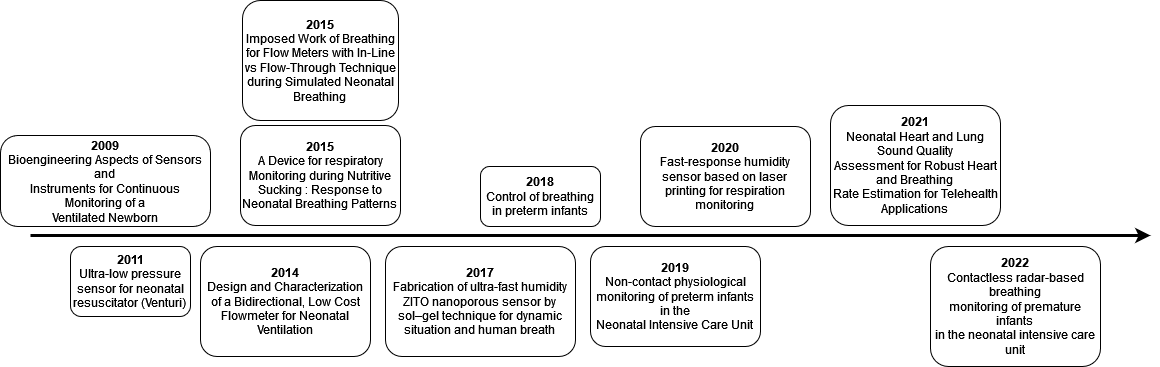
\includegraphics[scale = 0.3]{images/DRP_Etat_de_l_art.png}
    \caption{Articles scientifiques par ordre chronologique}
    \label{fig:articlesChrono}
\end{figure}

Les articles pertinants pour ce Travail de Bachelor sont résumés dans ce chapitre et classé par ordre chronologique sur la figure 
\ref{fig:articlesChrono}. \\

Le premier article \cite{rolfe_bioengineering_2009}, mentionne plusieurs débitmètres différents. Le pneumotacographe de Fleisch, par exemple, est un 
système par lequel le débit repiratoire est mesuré grâce à une différence de pression. Cette différence de pression est engendré par 
un rétrécissement de l'espace de circulation du gaz (principe de Venturi) \cite{oberg_biomedical_2011}. \\

Par la suite, il est expliqué que le pneumotachographe est gentiment remplacé par les anémomètres à fil chaud. Ces capteurs sont 
constitués d'un ou plusieurs fils chauffé par une source de courant. Lorsqu'un flux d'air va souffler sur le fil, la chaleur sera 
transférée du fil au gaz. Le capteur viendra alors mesurer la quantité de chaleur transférée ainsi que la différence de température entre 
le fil et le gaz pour finalement calculer le débit \cite{oberg_biomedical_2011}. \\
L'article sus-mentionné conseil l'utilisation des anémomètres à plusieurs fils contrairement à ceux à un seul fil qui aurait des performances 
moindres. 
L'anémomètre à fils chauds est une technologie incorporée par exemple dans la machine "Draeger Babylog", marque mentionnée dans le tableau \ref{tab:marques}. \\

Le second article exploite le principe de Venturi mentionné auparavant \cite{jacq_ultra-low_2011}. Il est destiné à une aplication 
quelques peu différente puisqu'il est  intégrer dans un ressuscitateur. Un tel appareil permet la réanimation du patient qui ne respire 
plus. Le ressuscitateur gonfle les poumons d'air et ainsi s'assure qu'un bon taux d'oxygène circule dans le patient. \\
Pour les nouveaux-né, la quantité d'air injectée dans les poumons doit être mesurée car un trop grand débit pourrait rapidement engendrer 
des dégats. \\
Couplé au système de Venturi, un capteur de force vient mesurer la pression et le volume d'air passant par le ressuscitateur. \\

Une autre technologie pour débitmètre consiste à utiliser le transfert de chaleur entre deux transistors. 
\begin{figure}[H]
    \centering
    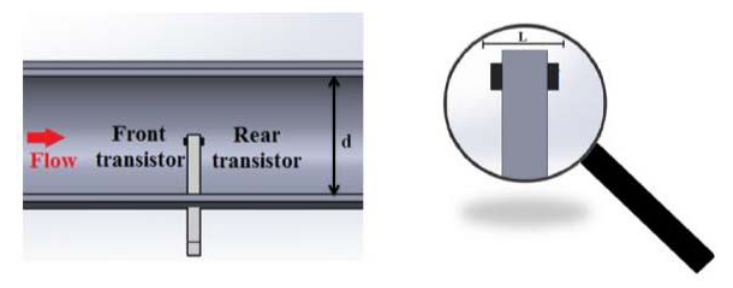
\includegraphics[scale = 0.5]{images/Debitmetre_transistors.png}
    \caption{Principe du débitmètre à transistors}
    \label{fig:transistors}
\end{figure}
C'est un principe encore innovant décrit dans l'article \cite{giorgino_design_2014} et utilisé dans l'article \cite{rosi_device_2016}. 
Le premier transistor est placé perpendiculairement au flux d'air sur un PCB. \\
Le second est fixé de l'autre côté du PCB dos à dos avec le premier transistor (cf. figure \ref{fig:transistors}). \\
De cette manière, le capteur sera capable de distinguer une expiration d'une inspiration. Le temps de réponse d'un tel capteur serait 
d'environ 340ms. C'est un très bon temps de réponse en comparaison des capteurs médicaux existants sur le marché. Cependant, diverses améliorations 
doivent encore être faites avant de pouvoir utiliser une telle technologie. \\

\begin{comment}
L'article suivant est intéressant au niveau du listage des débitmètres pédiatriques existants \cite{}. En effet, il étudie les différents fonctionnements 
existants et compare les signaux obtenus. Étant donné que cet article étudie plus précisément une caractéristique ("IN-line" vs "Flow-Through"), 
il est moins important dans le cadre de ce projet.\\
\end{comment}

Un autre article mentionne les membranes nanoporeuses comme capteur \cite{moharamzadeh_fabrication_2018}. Cependant, ces capteurs sont pour l'humidité et non le débit 
respiratoire. Des nanostructures d'oxyde de Zinc sont utilisées, car elles possèdes de bonnes propriétés physiques et chimiques. Bien que l'humidit 
et le débit respiratoire soient en lien, l'article n'a pas étudiés en détail l'application de cette membrane au débit respiratoire directement. \\
Cependant, un temps de réponse plutôt bon, de l'ordre de la seconde est attendu avec une telle technologie. \\

Le prochain article repose sur une technologie de monitoring non-invasive. Elle utilise une caméra qui suit les mouvements du nouveaux-né. 
Cette technologie permet également d'enregistrer d'autres signaux tels que la fréquence cardiaque mais elle requiert encore quelques améliorations 
ainsi que quelques recherches supplémentaires. 


\section{Un débitmètre innovant}
Ce travail de Bachelor est une recherche à propos d'un débitmètre dont le principe de fonctionnement est encore innovant. Il utilise des 
membranes nanoporeuses qui permettent une acquisition de données rapides. 

\section{Fonctionnement du débitmètre respiratoire pédiatrique}
Le capteur développé lors de ce Travail de Bachelor, repose sur le phénomène de l'effet Seebeck. Phénomène que l'on peut également retrouver 
dans les thermocouples. L'effet Seebeck est le suivant :\\
Lorsque deux matériaux conducteurs ou semi-conducteurs sont soumis à des températures différentes, une tension va être produite entre ces deux matériaux. \\
Sur la Figure \ref{fig:Seebeck}, deux matériaux sont côte à côte. Une source de chaleur vient chauffer le matériau de gauche. 
\begin{figure}[H]
    \centering
    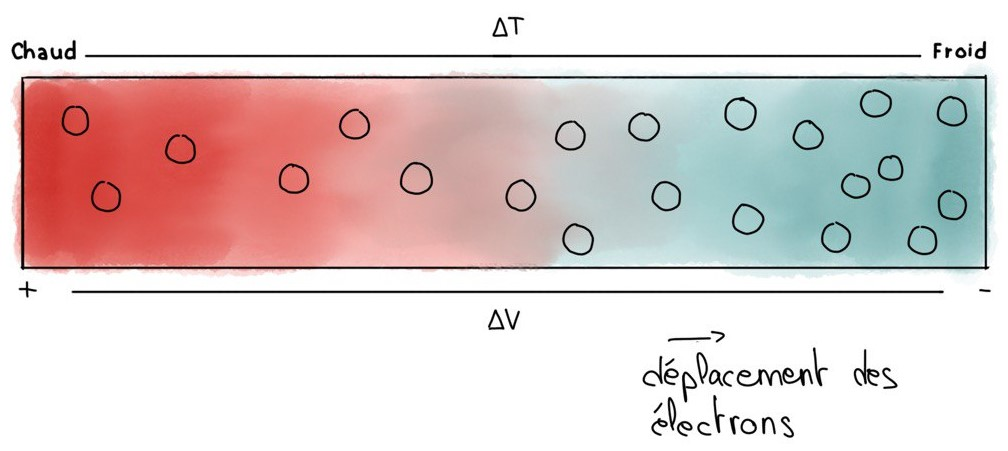
\includegraphics[scale = 0.3]{images/Seebeck.jpg}
    \caption{Effect de Seebeck}
    \label{fig:Seebeck}
\end{figure}
Les électrons au sein de la matière vont se déplacer du chaud vers le froid, créant ainsi un courant \cite{instrumentys_effet_2021}.\\
La tension est calculée grâce à la formule suivante :
\[V = S \cdot (T_{chaude} - T_{froide})\]
Avec S, le coefficient de Seebeck\\
Comme évoqué plus haut, le capteur est constitué de membranes nanoporeuses achetées sur le marché. 
Un côté de la membrane va être recouverte d'un matériau conducteur, l'or. Puis, Les pores de cette membrane sont remplies par 
électrodéposition avec une solution de Tellure de Bismuth (cf. figure \ref{fig:electrodeposition}). Ces pores remplis de tellure de 
Bismuth deviennent alors des nanofils. 
\begin{figure}[H]
    \centering
    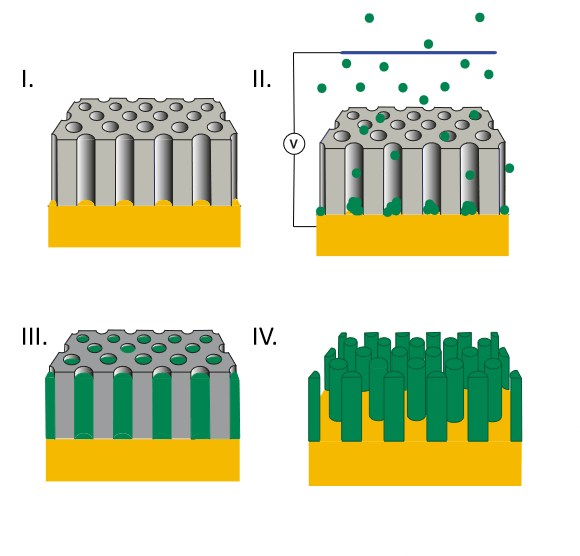
\includegraphics[scale = 0.5]{images/Electrodeposition.png}
    \caption{Electrodéposition \cite{ruiz-gomez_electrodeposition_2022}}
    \label{fig:electrodeposition}
\end{figure}

Le fonctionnement du débitmètre pédiatrique combine la technologie des nonofils et de l'effet de Seebeck. \\
En effet, un corps de chauffe est placé entre deux membranes nanoporeuses reliées entre elle par de l'or (bon conducteur). Une différence de 
température va se créer lorsque le patient viendra expirer ou inspirer de l'air sur le corps de chauffe (figure \ref{fig:CapteurFUN}). 
\begin{figure}[H]
    \centering
    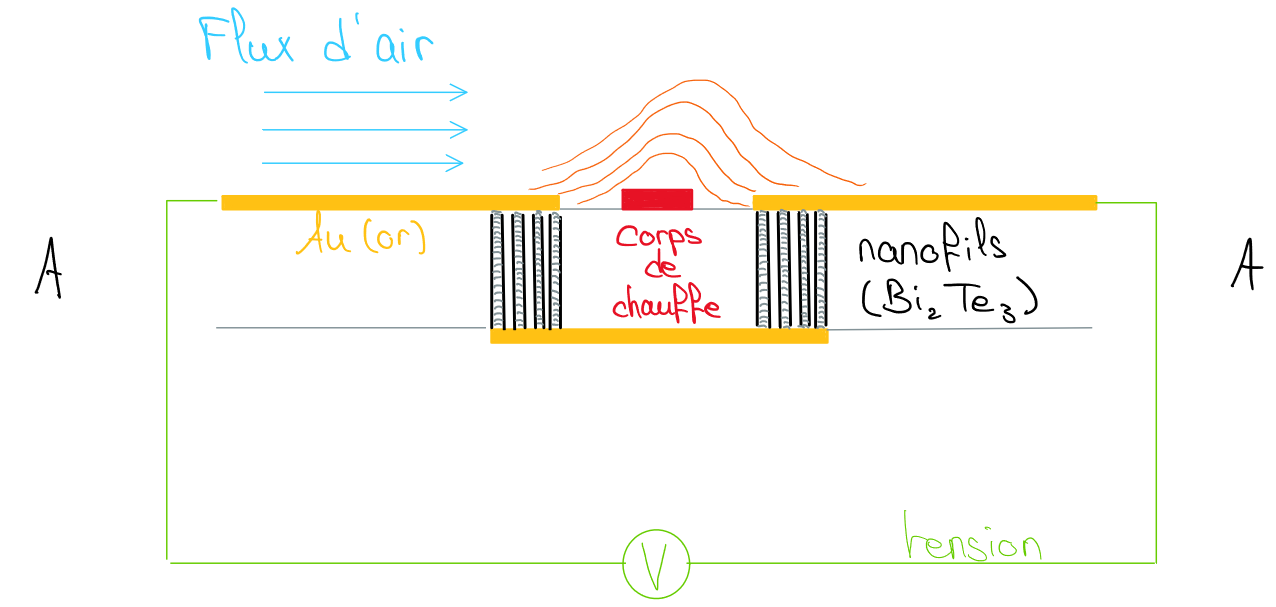
\includegraphics[scale = 0.7]{images/CapteurFUN.png}
    \caption{Schéma du débitmètre respiratoire pédiatrique}
    \label{fig:CapteurFUN}
\end{figure}
Nous pouvons observer sur la figure \ref{fig:CapteurFUN} que plusieurs électrodépositions ont été faites. Une première se situe à gauche 
du corps de chauffe et la deuxième, à sa droite. \\
Avec une différence de température de part et d'autre du corps de chauffe, un courant va circuler entre la couche d'or de gauche, à 
travers les nanofils gauches, au sein de la couche d'or du bas puis dans les nanofils de droite et une tension va apparaître. Il sera 
alors possible de lier cette tension au débit inspiré et expiré du nouveau-né.\\

Étant donné que les nanopores sont extrêmement fines et courtes, il est attendu d'obtenir un temps de réponse très intéressant (temps 
de réponse faible). 

\section{Cahier des charges}

\section{Livrables}

\section{Planification}

\section{Plan du rapport}

%%if
\section{Citations et bibliographie}
Citer vos sources est essentiel. Avec \texttt{biblatex} vous pouvez facilement citer des articles, des livres ou des sites internet. Toutes les citations dans le texte seront automatiquement regroupées en fin de document dans la section \guillemotleft Bibliographie\guillemotright. Par exemple, citons un article d'Einstein \cite{einstein} ou le livre de Dirac \cite{dirac}.

Parfois il peut être utile d'utiliser un gestionnaire de bibliographie. La communauté académique recommande l'outil \href{https://www.zotero.org/}{Zotero} qui permet de gérer une bibliothèque numérique d'ouvrages et de références numériques. Il permet également de générer une bibliographie compatible avec \LaTeX.

Notez qu'il est très facile d'obtenir l'extrait \texttt{bibtex} depuis des journaux. Sélectionnez \emph{export/citation}. Si vous le pouvez choisissez \texttt{bibtex}. Dans le cas d'un format \texttt{.ris}, utilisez un convertisseur en ligne comme \href{http://www.bruot.org/ris2bib/}{ris2bib}.

\section{Adapter votre modèle}
Ce document n'est qu'un modèle ayant pour but de revoir les quelques avantages de \LaTeX~ et les fonctionnalités qui pourraient vous être utiles pour rédiger un rapport académique. N'hésitez pas à supprimer les parties inutiles et à adapter ce modèle à vos besoins.
%%fi
%%%if
\section{Exemple d'équation}
L'une des principales forces de \LaTeX~est la saisie d'équations. L'équation \ref{eq:1}, citée à titre d'exemple, représente la transformation de phase d'une lentille biconvexe. Pour rédiger une équation \LaTeX~vous pouvez utiliser des outils en ligne tels que \href{https://www.latex4technics.com/}{latex4technics}. Essayez autant que possible d'écrire vos équations à la main. La courbe d'apprentissage n'est pas très raide et la valeur ajoutée est grande. Vous pouvez vous aider du panneau de \LaTeX~Workshop dans Visual Studio Code. Il est accessible via le raccourcis clavier \keystroke{Ctrl} + \keystroke{Alt} + \keystroke{X}.

\begin{equation} \label{eq:1}
    \begin{split}
        L(x,y) &= \exp\left( - i\frac{{2\pi }}{\lambda }\left( {n\Delta \varphi (x,y) + \Delta {\varphi _0} - \Delta \varphi (x,y)} \right)\right)\\
        &= {\exp\left({i\frac{{2\pi }}{\lambda }\Delta {\varphi _0}}\right)}{\exp\left({ - i\frac{{2\pi }}{{\lambda f}}({x^2} + {y^2})}\right)}
    \end{split}
\end{equation}

\section{Exemples de diagrammes}

Les diagrammes de flux peuvent être réalisés en utilisant l'outil \href{https://app.diagrams.net/}{draw.io}. Une exportation en \texttt{.drawio} (non compressé) permet de garder les sources de la figure. Le rendu en \texttt{.pdf} sera réalisé à la volée à la compilation. L'intérêt est double : n'avoir qu'une source de vérité \cad pas d'image intermédiaire à stocker, et réduire la quantité d'information stockée.

Puisque la source est au format XML, les textes sont accessibles au correcteur orthographique et il vous est rendu possible les modifier sans avoir à éditer l'image. La figure \ref{euclide.drawio} en est un exemple.

\fig[H, width=9cm]{Algorithme d'Euclide}{euclide.drawio}

Notons qu'il est inutile d'insérer des images coloriées là où la couleur n'offre aucune valeur ajoutée ; évitez également les ombrages et autres effets de style. Enfin, préférez toujours des représentations vectorielles là où c'est possible.

Voici un autre type de diagramme utile (figure \ref{sequence.drawio}), celui d'une séquence UML.

\fig[H, width=0.4\textwidth]{Diagramme de séquence}{sequence.drawio}

Ce modèle apporte la commande \verb!\fig! qui peut prendre plusieurs options. Utilisez \verb!H! pour forcer la figure à apparaître à l'endroit de la déclaration. Ajustez la largeur de la figure à \SI{80}{\percent} de largeur de page avec \verb!width=0.8\textwidth!.

\section{Exemple de figure}

Pour présenter vos résultats d'expérience, vous pouvez soit dessiner des graphiques manuellement en utilisant des outils de dessin vectoriel comme Inkscape ou Adobe Illustrator, comme illustré à la figure \ref{plot.svg}.

\fig[H, width=0.8\textwidth]{Exemple de graphique plan}{plot.svg}

Vous pouvez utiliser Python ou Matlab pour générer des figures à la volée à partir d'une source de données. À titre d'exemple, le code source \ref{python} permet de générer la figure \ref{bode.py}.
\begin{listing}[h]
    \inputminted{python}{assets/figures/bode.py}
    \caption{Génération d'un diagramme de Bode \label{python}}
\end{listing}

\fig[H, width=12cm]{Diagramme de Bode généré à la volée}{bode.py}

\subsection{Example de schéma électronique}
Vous pouvez également utiliser TikZ pour créer vos propres schémas électriques et électroniques comme l'exemple \ref{circuit}. N'hésitez pas à vous inspirer d'exemples disponibles sur internet (\href{https://texample.net/tikz/examples/area/electrical-engineering/}{texample/electrical-engineering}).

\begin{figure}[h]
    \begin{center}
        \begin{circuitikz}
            \draw
            (0,0) to [short, *-] (6,0)
            to [V, l_=$\mathrm{j}{\omega}_m \underline{\phi}^s_R$] (6,2)
            to [R, l_=$R_R$] (6,4)
            to [short, i_=$\underline{i}^s_R$] (5,4)
            (0,0) to [open, v^>=$\underline{u}^s_s$] (0,4)
            to [short, *- ,i=$\underline{i}^s_s$] (1,4)
            to [R, l=$R_s$] (3,4)
            to [L, l=$L_{\sigma}$] (5,4)
            to [short, i_=$\underline{i}^s_M$] (5,3)
            to [L, l_=$L_M$] (5,0);
        \end{circuitikz}
        \caption{Circuit électrique \label{circuit}}
    \end{center}
\end{figure}

\subsection{Dessins techniques}
La présentation de dessins mécaniques est préférée en vue filaire. SolidWorks conserve la représentation vectorielle à l'exportation mais pas lorsqu'il y a des textures ou des rendus. À partir du PDF généré, l'image peut être isolée et sauvegardée en format SVG.

\begin{figure}[!ht]
    \begin{center}
        \includegraphics[width=10cm]{\assetsdir/assembly.svg.pdf}
    \end{center}
    \caption[Assemblage mécanique]{\label{assembly}Réducteur cycloïdale de puissance comportant 6. l'axe de sortie, 14. le roulement de sortie, 1. le corps du réducteur en aluminium, 3 et 5. les disques cycloïdaux et 2. les goupilles de prise... D'autres informations liées à la figure elle-même peuvent aussi figurer dans la légende}
\end{figure}

Notez ici que la légende est particulièrement longue. Celle que vous retrouverez dans la table figures est plus courte. La commande \mintinline{latex}{\caption[courte]{longue}} permet de saisir une légende courte pour la table des figures et une légende longue pour documenter la figure. Utilisez \mintinline{latex}{\fig[short=Légende courte]{Légende longue}{fichier}}.

La figure \ref{assembly} est un dessin technique épuré qui permet de décrire un phénomène ou un fonctionnement important dans le rapport technique. Les mises en plan détaillées seront quant à elles disponibles en annexes.

\section{Tableaux}

Concernant les tableaux un seul conseil : restez simple et minimaliste, n'ajoutez des séparateurs que là ou c'est nécessaire pour améliorer la lisibilité. Une liste de quelques cantons suisses est donnée à titre d'exemple dans la table \ref{cantons}.

\begin{table}[h]
    \begin{center}
        \caption{Liste des cantons \label{cantons}}
        \begin{tabular}{c|l|r}
            Abréviation & Nom du canton & Depuis                  \\ \hline
            ZH          & Zürich        & \ordinalnum{1} mai 1351 \\
            BE          & Berne         & 6 mars 1353             \\
            FR          & Fribourg      & 22 décembre 1481        \\
            VD          & Vaud          & 19 février 1815         \\
            VS          & Valais        & 4 août 1815             \\
            NE          & Neuchâtel     & 19 mai 1815             \\
            GE          & Genève        & 19 mai 1815
        \end{tabular}
    \end{center}
\end{table}

Comparez la lisibilté de cette même table avec celle que vous pourriez trouver dans un document Word :

\begin{table}[h]
    \begin{center}
        \caption{Liste des cantons (vilain)}
        \begin{tabular}{|l|l|l|} \hline
            \textbf{Abréviation} & \textbf{Nom du canton} & \textbf{Depuis}         \\
            \Xhline{4\arrayrulewidth}
            ZH                   & Zürich                 & \ordinalnum{1} mai 1351 \\ \hline
            BE                   & Berne                  & 6 mars 1353             \\ \hline
            FR                   & Fribourg               & 22 décembre 1481        \\ \hline
            VD                   & Vaud                   & 19 février 1815         \\ \hline
            VS                   & Valais                 & 4 août 1815             \\ \hline
            NE                   & Neuchâtel              & 19 mai 1815             \\ \hline
            GE                   & Genève                 & 19 mai 1815             \\ \hline
        \end{tabular}
    \end{center}
\end{table}

Si vous devez donner une spécification technique, n'oubliez pas de mentionner les valeurs minimales, maximales et nominales sans omettre l'unité de mesure. Notez que les séparateurs verticaux sont souvent critiqués pour réduire la lisibilité mais parfois ils sont utiles. Utilisez-les avec parcimonie. Jouez avec l'alignment des colonnes pour accroître la lisibilité et utilisez l'environmement \mintinline{latex}{tabularx} pour plus d'unité dans les largeurs de vos tableaux.

\begin{table}[h]
    \begin{center}
        \caption{Exigences techniques \label{specification}}
        \begin{tabularx}{\textwidth}{cXcccr}
            \toprule
            No. & Exigence                                                                   & Min. & Nom. & Max. & Unité                           \\
            \midrule
            E1  & Tension d'alimentation                                                     & 12   & 24   & 48   & \si{\volt}                      \\
            E2  & Fréquence                                                                  & 50   &      & 60   & \si{\hertz}                     \\
            E3  & Concentration                                                              &      & 300  & 1200 & \si{\nano\gram\per\milli\litre} \\
            E4  & \multicolumn{5}{l}{Doit pouvoir être stoppé à l'aide d'un arrêt d'urgence}                                                        \\
            \bottomrule
        \end{tabularx}
    \end{center}
\end{table}

L'exemple de la table \ref{specification}, assigne pour chaque exigence un numéro unique. Cette table est \textbf{normative}, chaque élément doit pouvoir être référencé par un identifiant unique (cf. T\ref{specification}-E3). Dans le cas ou cet identifiant est utilisé en dehors de ce document, la version du document devra être renseignée.

\section{Index}
\LaTeX~ permet d'indexer les mots \index{mots} importants. Il suffit de placer les termes importants d'un paragraphe dans la commande \mintinline{latex}{\index{terme}} et ils apparaîtront automatiquement à la fin de ce rapport dans l'index du document.

\index{Napoléon}

Imaginons que dans cette section nous parlions du cheval blanc \index{cheval blanc} de Napoléon. Il se pourrait que le lecteur recherche ce passage dans la version imprimée du rapport. Avec l'index, rien de plus facile. Allez jeter un oeil à la page \pageref{index}.

\section{Notes de bas de page}

\maraja{Je suis une marginale, et je suis utile pour résumé un paragraphe en quelques mots.} Parfois, il est plus élégant d'annoter une définition en utilisant une note de bas de page \footnote{La note en bas de page (ou note de bas de page) est une forme littéraire, consistant en une ou plusieurs lignes ne figurant pas dans le texte.}. Alternativement il est possible d'annoter un paragraphe avec une note marginale.

\section{Glossaire et acronymes}

La \Gls{heig-vd} membre de la \Gls{hes-so} propose ce modèle de document. Le format \LaTeX~est particulièrement adapté pour les documents qui contiennent des expressions mathématiques. Pour plus de détail sur l'utilisation d'un glossaire, se référer à \href{https://www.overleaf.com/learn/latex/Glossaries}{Overleaf/Glossaires}. Tient donc, ci-dessus nous utilisons deux acronymes. Les trouverez-vous dans le glossaire en page \pageref{glossaire} ?

\section{Unités de mesure}

Lorsque vous mentionnez des quantités, utilisez les unités du système international. \LaTeX~et le paquet \texttt{siunitx} permet la saisie de quantités. La commande suivante permet d'afficher \SI{42.12}{\kilo\gram\metre\per\square\second}.\par

\mintinline{latex}{\SI{42.12}{\kilo\gram\metre\per\square\second}}\par

Notez qu'une espace fine précède l'unité et que ces dernières ne sont pas en italiques.
%%fi

\chapter{Fabrication des capteurs FUNs}
\section{Méthode de fabrication du capteur}
\label{chap:capteur}
Le capteur constitué de la membrane nanoporeuse, des électrodépositions ainsi que des dépôts physiques en phase vapeur d'or (PVD) sont 
fabriquées avec plusieurs membranes différentes et selon 2 méthodes :

\subsection{Membranes à disposition}
\begin{table}[H]
    \begin{tabular}{|c|c|}
        \hline
        Matériau de la membrane & Épaisseur de la membrane \\
        \hline
        GTTP                    & 6 à 10 $\mu m$           \\
        \hline
        VCTP                    & 6 à 10 $\mu m$           \\
        \hline
        PI25005                 & 25 $\mu m$               \\
        \hline
    \end{tabular}
    \caption{Matériau des membranes disponibles}
\end{table}

\subsection{Dénomination des échantillons}
\begin{table}[H]
    \centering
    \begin{tabular}{|c|c|c|}
        \hline
        Échantillon & Membrane & Méthode d'électrodéposition \\
        \hline
        D06         & GTTP     & A                           \\
        \hline
        D12         & PI25005  & A                           \\
        \hline
        D13         & PI25005  & B                           \\
        \hline
        D14         & VCTP     & A                           \\
        \hline
    \end{tabular}
    \caption{Dénomination des échantillons}
\end{table}

\subsection{Méthode A et B}
Les méthodes d'électrodéposition correspondent à la définition suivante :
\begin{itemize}
    \item Méthode A
          \begin{figure}[H]
              \hspace{-0.5cm}
              \begin{subfigure}{0.45\textwidth}
                  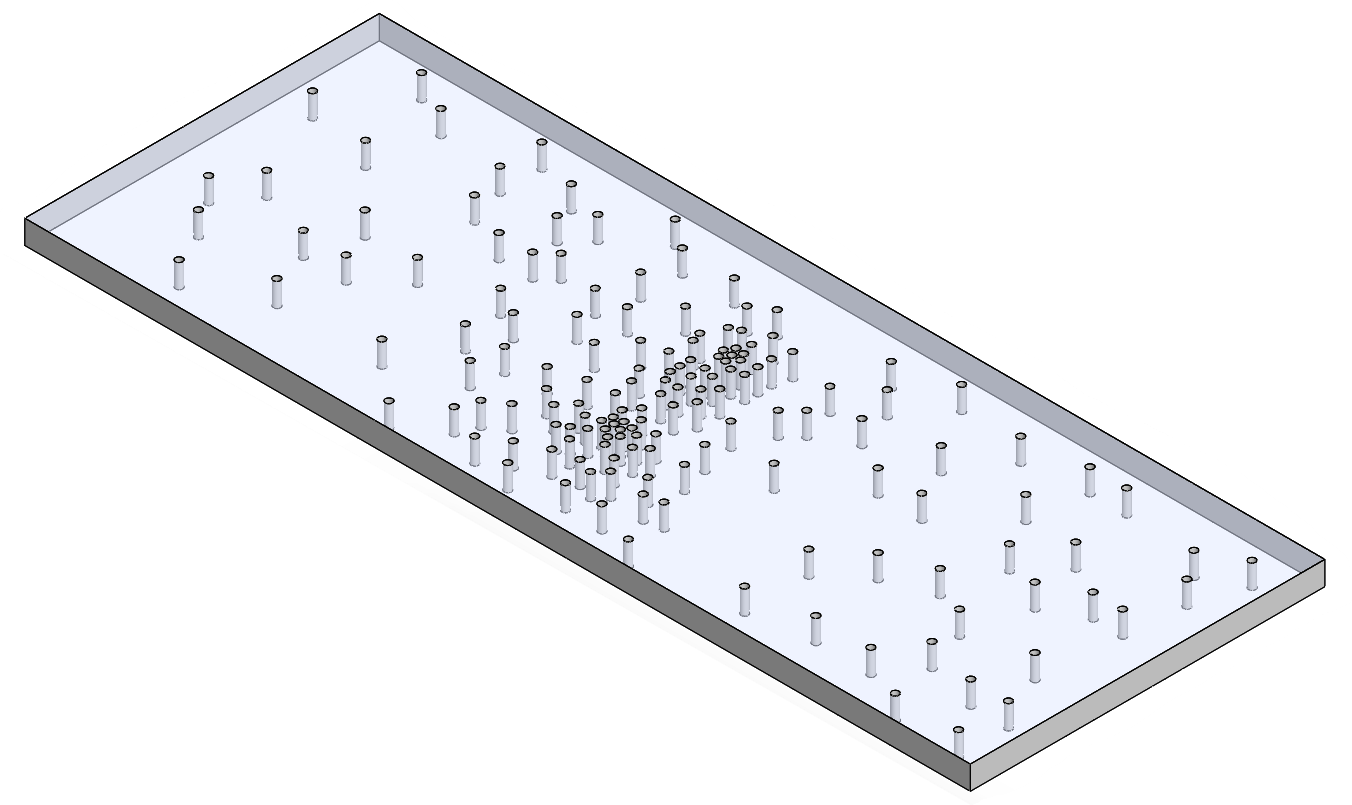
\includegraphics[scale = 0.25]{assets/figures/Membrane_nue.png}
                  \caption{Membrane nanoporeuse}
              \end{subfigure}
              \begin{subfigure}{0.45\textwidth}
                  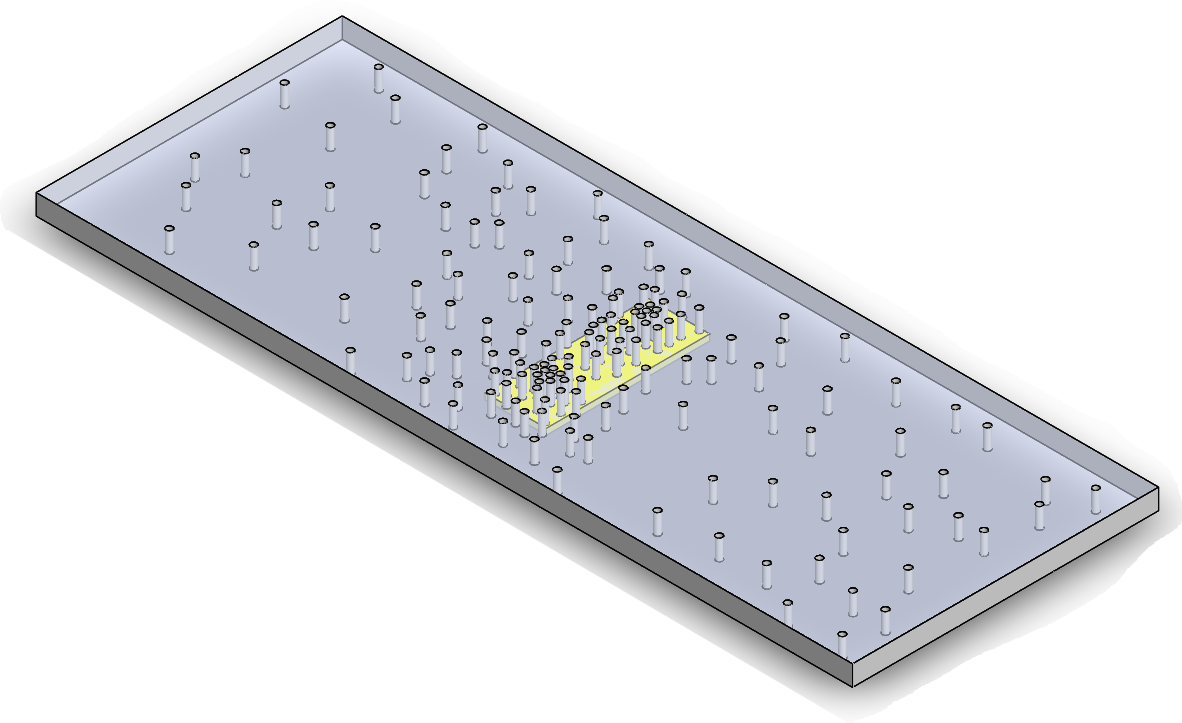
\includegraphics[scale = 0.3]{assets/figures/Court_circuit.png}
                  \caption{Dépôt physique en phase vapeur (PVD) d'or du court-circuit}
              \end{subfigure}
              \newline
              \begin{subfigure}{0.45\textwidth}
                  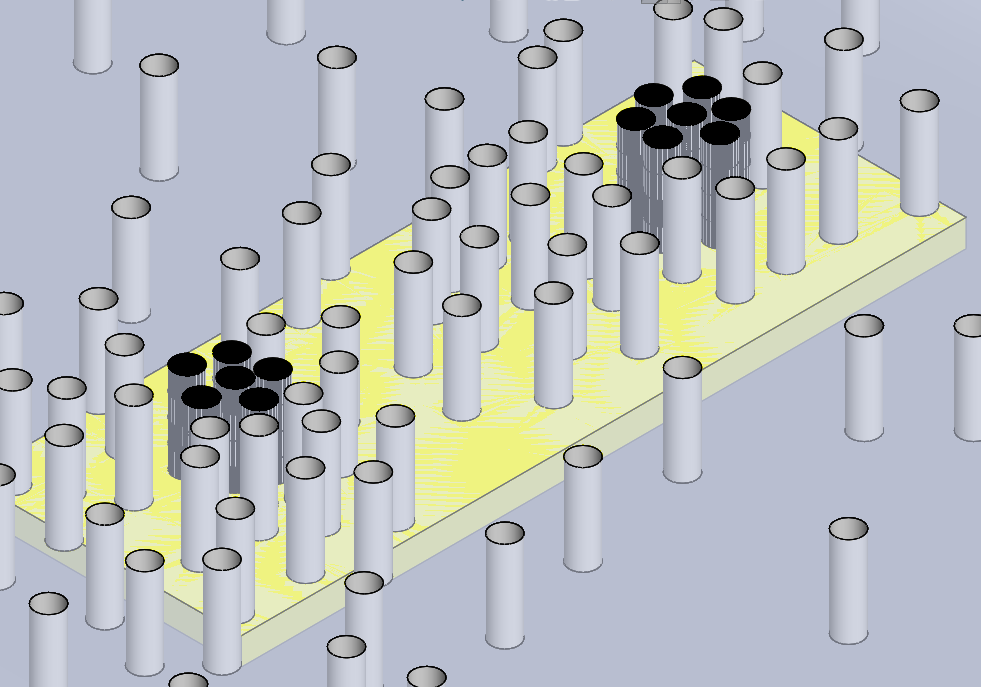
\includegraphics[scale = 0.3]{assets/figures/ED.png}
                  \caption{Électrodépositions effectuées un côté après l'autre}
              \end{subfigure}
              \begin{subfigure}{0.45\textwidth}
                  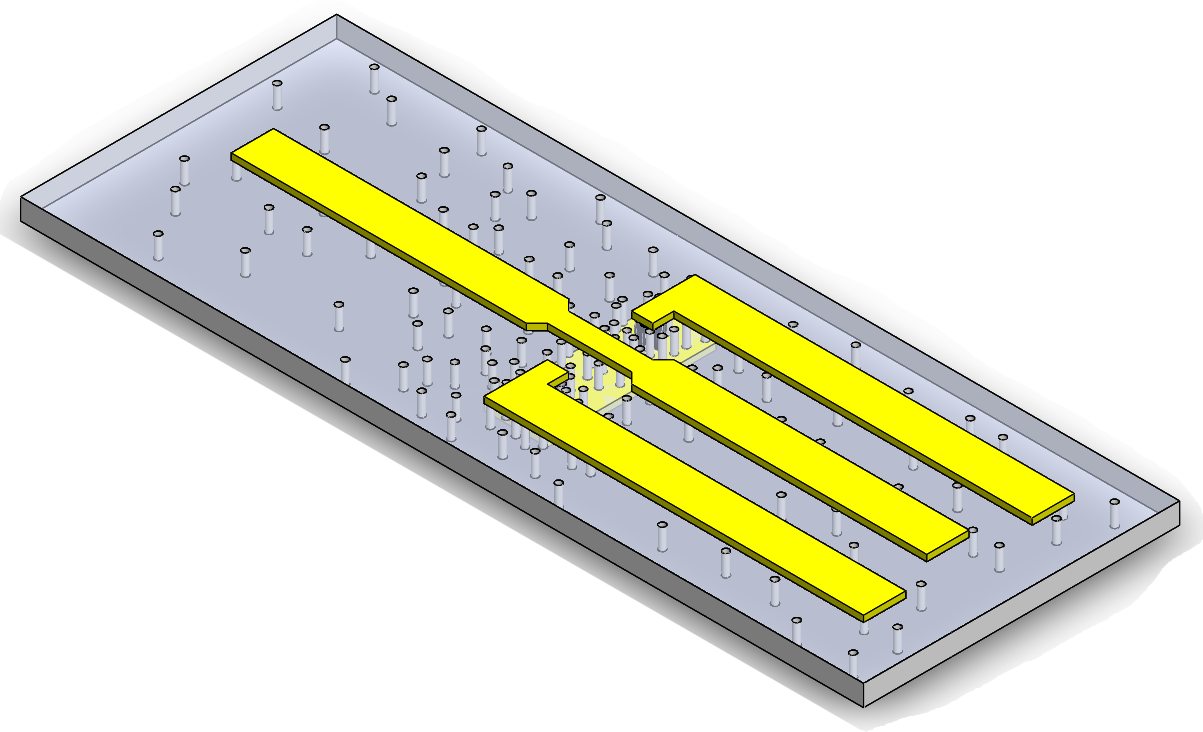
\includegraphics[scale = 0.3]{assets/figures/PVD_L.png}
                  \caption{PVD d'or des branches en L}
              \end{subfigure}
          \end{figure}
    \item Méthode B
          \begin{figure}[H]
              \hspace{-0.5cm}
              \begin{subfigure}{0.45\textwidth}
                  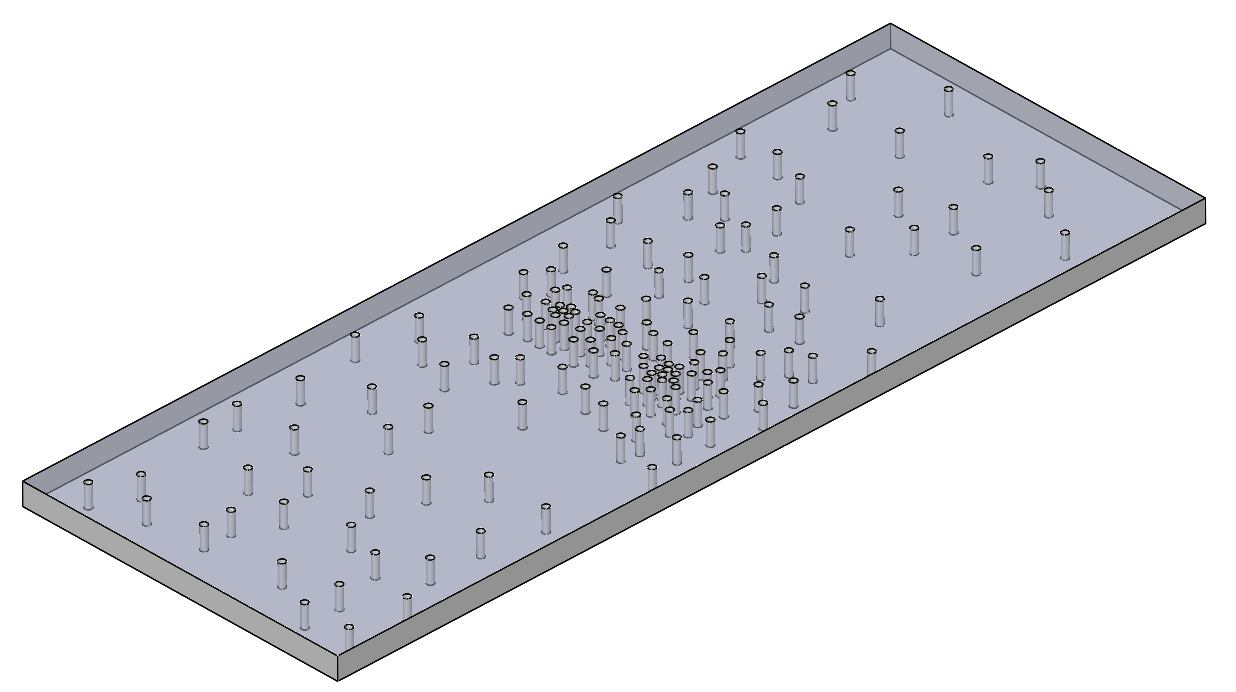
\includegraphics[scale = 0.3]{assets/figures/Membrane_nue_B.png}
                  \caption{Membrane nanoporeuse}
              \end{subfigure}
              \begin{subfigure}{0.45\textwidth}
                  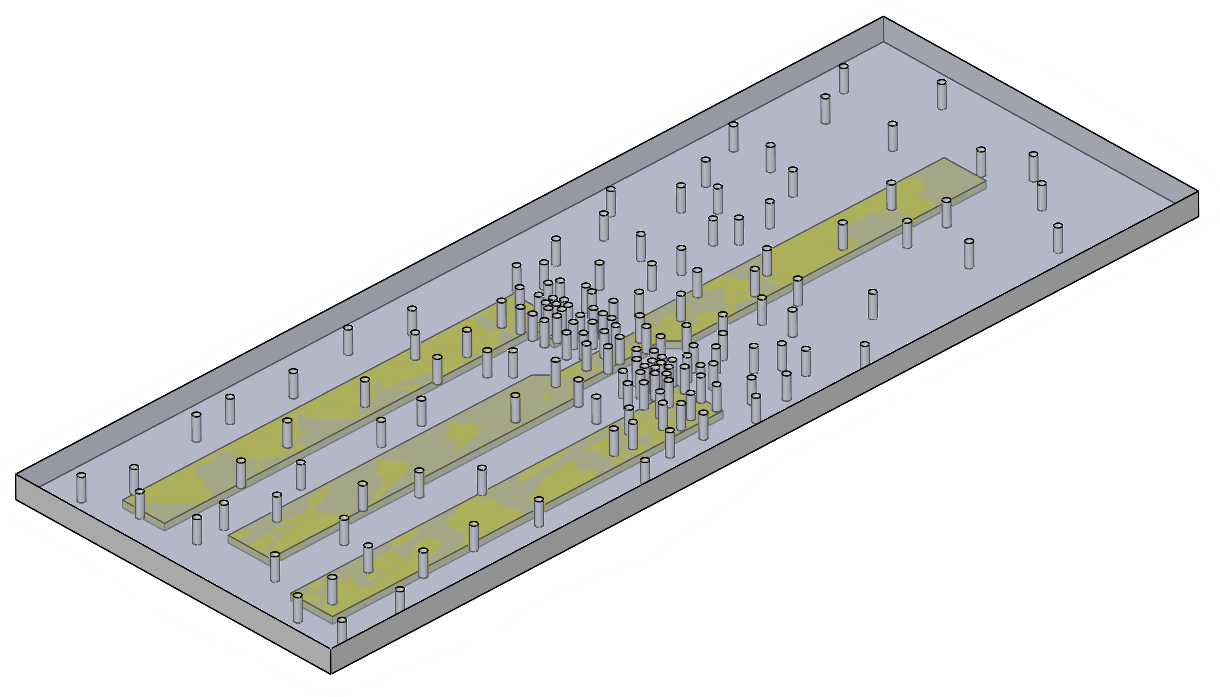
\includegraphics[scale = 0.3]{assets/figures/PVD_L_B.png}
                  \caption{PVD d'or des branches en L}
              \end{subfigure}
              \newline
              \begin{subfigure}{0.45\textwidth}
                  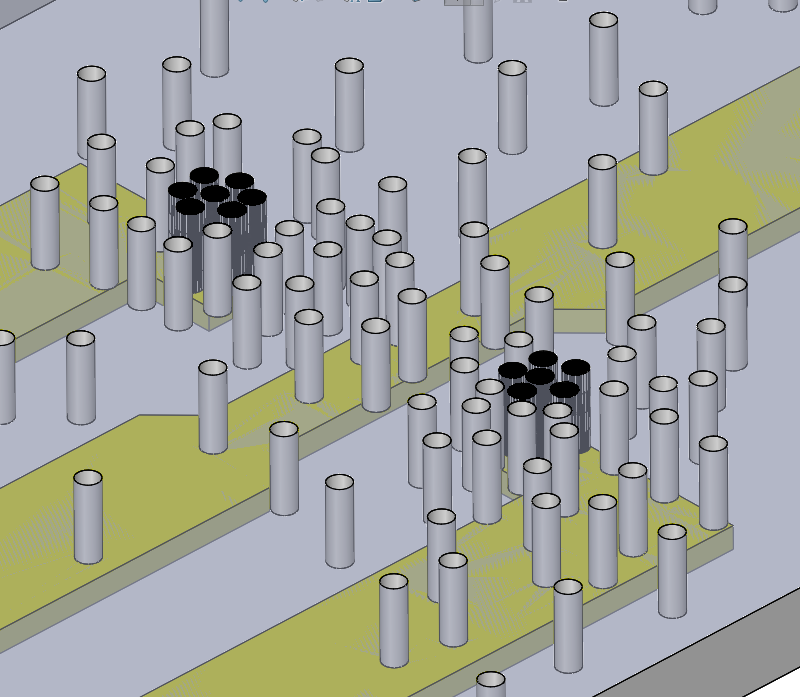
\includegraphics[scale = 0.3]{assets/figures/ED_B.png}
                  \caption{Électrodépositions effectuées une après l'autre}
              \end{subfigure}
              \begin{subfigure}{0.45\textwidth}
                  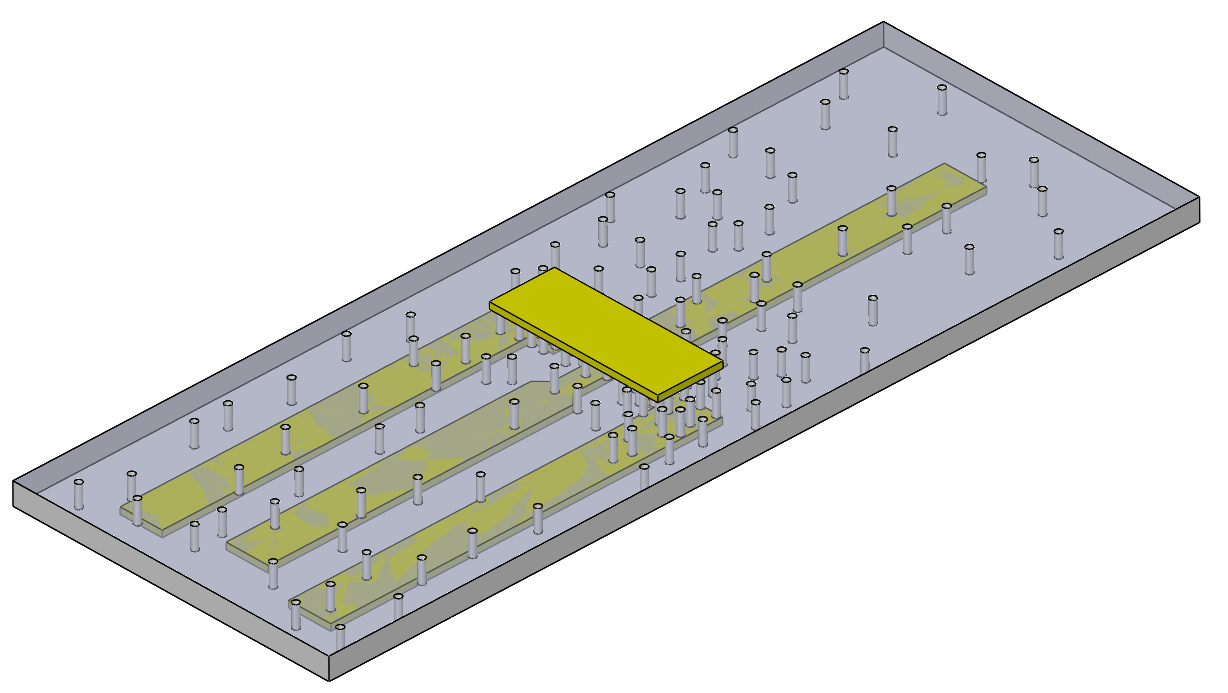
\includegraphics[scale = 0.3]{assets/figures/Court_circuit_B.png}
                  \caption{PVD d'or du court-circuit}
              \end{subfigure}
          \end{figure}
\end{itemize}

\section{Catalogue des solutions du support}
\label{chap:catalogueSol}
Plusieurs systèmes ont été étudiés afin d'incorporer le capteur dans une conception permettant de connecter les membranes et le corps de chauffe
ainsi que d'y attacher un système apportant un flux d'air (imitation de la respiration du patient). Ces différentes solutions seront appeléess
"Support des capteur \gls{capteur}s".

\subsection{Design 1}
\begin{figure}[H]
    \centering
    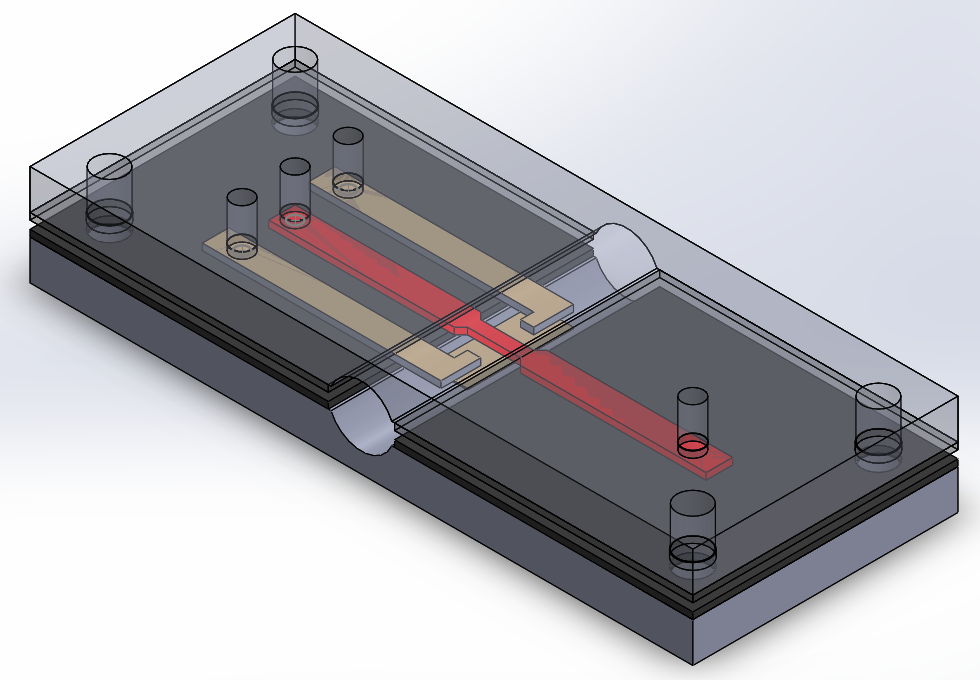
\includegraphics[scale = 0.3]{images/Design1.png}
    \caption{Design 1}
    \label{fig:design1}
\end{figure}
Ce premier design est le plus basique. Il vient plaquer le capteur entre deux couches presque semblables. Sur une des couches se trouvent des
perçages permettant de tenir des contacts à ressorts (pointes ressorts). Celles-ci viennent s'appuyer d'un côté sur le capteur et
de l'autre, une  connection pourra être faite par des pinces crocodiles ou des soudures. \\
Un joint plat peut venir de part et d'autre du capteur afin d'assurer l'étanchéité du système.\\
Cette solution a le désavantage d'avoir une arrivé d'air scindée en deux. Le placement ainsi que l'étanchéité au niveau de l'entrée
d'air risque d'être mauvaise. \\
Ceci mis de côté, c'est une solution simple, rapide et compacte.

\subsection{Design 2}
Afin d'éviter l'entrée d'air scindée en deux, une solution pourrait être celle représentée ci-dessous :
\begin{figure}[H]
    \centering
    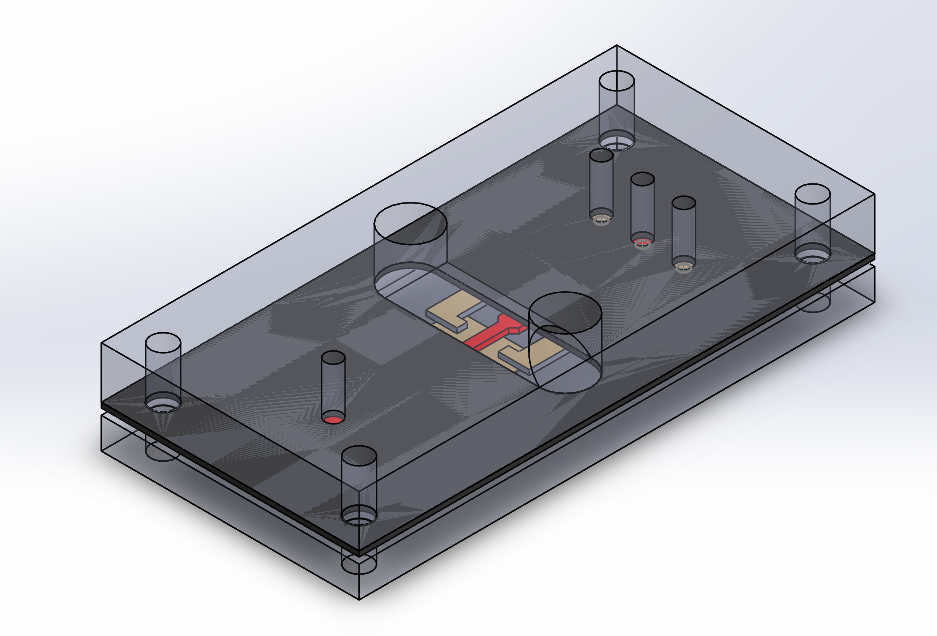
\includegraphics[scale = 0.3]{images/Capteur_design2_caoutch.png}
    \caption{Design 2}
    \label{fig:design2}
\end{figure}
L'arrivée d'air se fait par le haut du système et est dévié par la suite afin d'arriver sur le capteur. Cette solution permet d'avoir une
entrée d'air plus régulière et utilisable que la solution précédente. Cependant, elle ajoute un risque non-négligeable au niveau des turbulences. En effet,
les coudées risquent d'engendrer des turbulences au niveau du flux qui pourraient altérer les résultats.\\
Une particularité à noter est le fait que la membrane se retrouve entièrement plaquée contre une surface contrairement à la solution
précédante où le centre de la membrane (là où est situé le capteur), "flotte" au milieu du flux d'air.

\subsection{Design 3}
Une manière de diminuer les turbulences seraient d'élargir le système afin que les coudées ne se retrouvent pas trop proches de la
membrane.

\begin{figure}[H]
    \centering
    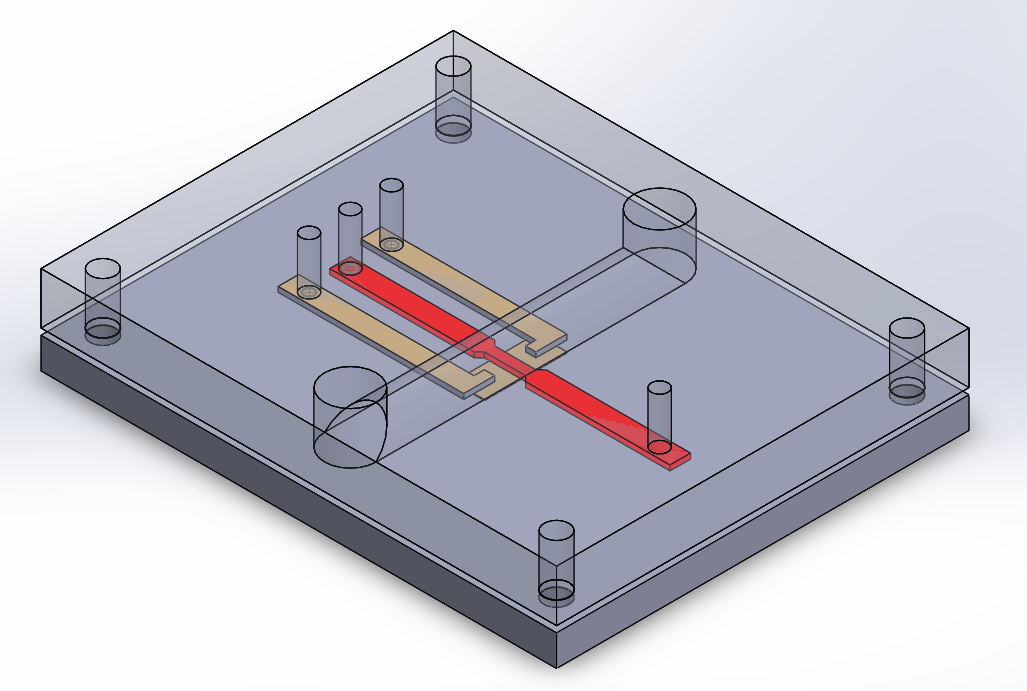
\includegraphics[scale = 0.3]{images/Design4}
    \caption{Design 3}
    \label{fig:design4}
\end{figure}

\begin{comment}
\section{Design 4}
Une autre manière d'éviter ce problème de turbulences et de changer la conception. Ainsi, le capteur pourrait être fabriqué selon la
figure \ref{fig:design6}.

\section{Design 4}%à effacer
\begin{figure}[H]
    \centering
    \includegraphics[scale = 0.5]{images/Design6}
    \caption{}
    \label{fig:design6}
\end{figure}

Cependant cette solution engendre un nombre de pièces plus élevé que les designs précédents. En effet, pour un conception comme celle
de la figure \ref{fig:design6}, 4 pièces seraient nécessaires contre 2 pièces pour les solutions précédentes.\\
Deux pièces viendraient pincer le capteur en sandwich comme montré pour le design 1, figure \ref{fig:design1}, puis, deux autres pièces
viendraient se poser sur les deux longueurs du système afin de permettre de conncter facilement une arrivée d'air.
\end{comment}

\subsection{Design 4}
Finalement, une dernière conception a été imaginée :
\begin{figure}[H]
    \centering
    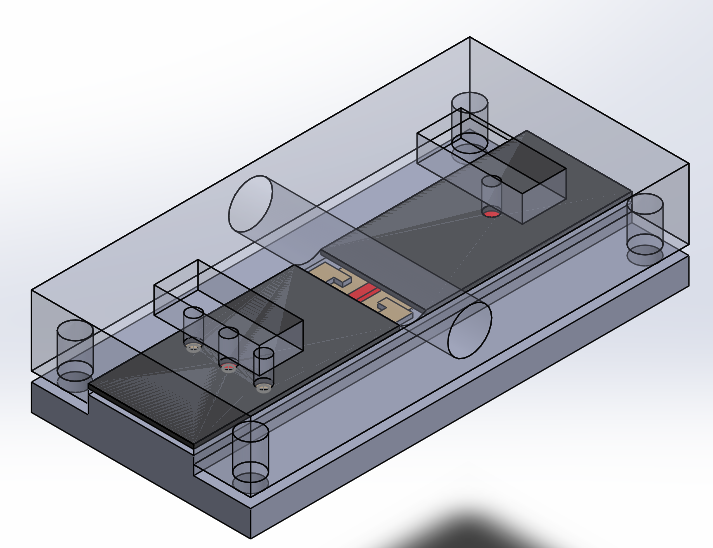
\includegraphics[scale = 0.4]{images/Design5_int_caoutch.png}
    \caption{Design 4}
    \label{fig:design5}
\end{figure}

Cette dernière permettrait de garder une solution à deux pièces seulement et incorporerait une entrée et une sortie d'air facilitée
(non-scindée en deux).\\
La membrane (capteur) posée sur une première pièce légèrement surrélevée. Un joint plat d'échantéité viendrait sur la membrane (en noir
sur la figure). Puis, une seconde pièce viendrait s'appuyer en sandwich contre le joint et le capteur. Cette pièce, sur le dessus, est
percée afin d'amener le flux d'air au niveau du capteur. Des plus petits perçages ainsi que des espaces creusés dans la pièce du dessus
permettent aux pointes ressorts de venir se poser sur la membrane afin d'assurer la connection électrique.\\

Finalement, deux designs ont été retenus. Le Design 1 ainsi que le Design 5. Ces deux designs vont être testés afin de mesurer la
performance d'un capteur recevant un flux d'air depuis le haut et depuis le bas simultanément ainsi qu'un capteur ne recevant un flux
d'air seulement par le haut (car le capteur est plaqué contre une surface).

\chapter{Banc de test}

\section{Spécifications}
Le banc de test doit suivre les spécifications suivantes :
\begin{itemize}
    \item Présence d'un débitmètre de référence permettant de connaître le flux entrant ou sortant du capteur
    \item Système permettant de tester les deux modèles de support de capteur (Solution 1 et 5)
    \item Échantillon de capteur \gls{capteur} fabriqué selon le circuit imposé (pistes en "L", piste de court-circuit, etc.)
    \item Échantillon de capteur \gls{capteur} facilement interchangeable
    \item Utilisation de l'air comprimé de la \gls{heig-vd} en air continu et/ou en air pulsé
\end{itemize}

\section{Types de sortie}
Quel que soit le banc de test réalisé, il y aura deux types de sorties possibles. \\

La première sortie vient mesurer directement sur le capteur 
\gls{capteur} (par le biais du support de capteur) la tension circulant dans le circuit thermoélectrique. Cette tension sera reportée dans un 
programme LabView qui viendra dessiner un graphe de la tension en fonction du temps. \\

Le deuxième type de sortie utilise un amplificateur de tension. La sortie en tension du capteur \gls{capteur} passe dans un amplificateur avant 
d'être affichée à l'oscilloscope. 


\section{Présentation des composants}
Le banc de test permet de tester de manière efficace le capteur \gls{capteur} en utilisant différents composants électroniques et appareils de 
mesures. Pour ce banc de test, le matériel suivant est utilisé :
\begin{itemize}
    \item \textbf{Capteur avec son support (Solution 1 ou 5)}\\
          La géométrie générale du Design 1 et 5 est expliquée et représentée au chapitre \ref*{chap:catalogueSol}. \\
          
    \item \textbf{Alimentation de laboratoire}\\
          Elle fournit la tension nécessaire au débitmètre de référence, à l'électrovanne et au corps de chauffe si ce dernier chauffe de manière 
          continue. \\
          
    \item \textbf{Générateur de fonctions}
          Le générateur de fonctions permet d'alimenter le corps de chauffe de manière cadencée. \\
          
    \item \textbf{Oscilloscope}\\
          Cet appareil permet d'observer le signal analogique du débitmètre de référence ainsi que le signal du capteur \gls{capteur}. \\
          
    \item \textbf{Débitmètre de référence FESTO SFAH-10B-Q6S-PNLK-PNVBA-M8}\\
          Le débitmètre choisi est un débitmètre bidirectionnel avec une entrée d'air de 6 mm de diamètre. Il sera placé juste avant l'entrée du flux
          d'air dans le capteur, permettant ainsi d'avoir une valeur de référence fiable.\\
          
          Un graphe de la tension en fonction du débit a été construit grâce à la sortie analogique du débitmètre de référence :
          \begin{figure}[H]
              \hspace{-1cm}
              \begin{subfigure}{0.4\textwidth}
                  \centering
                  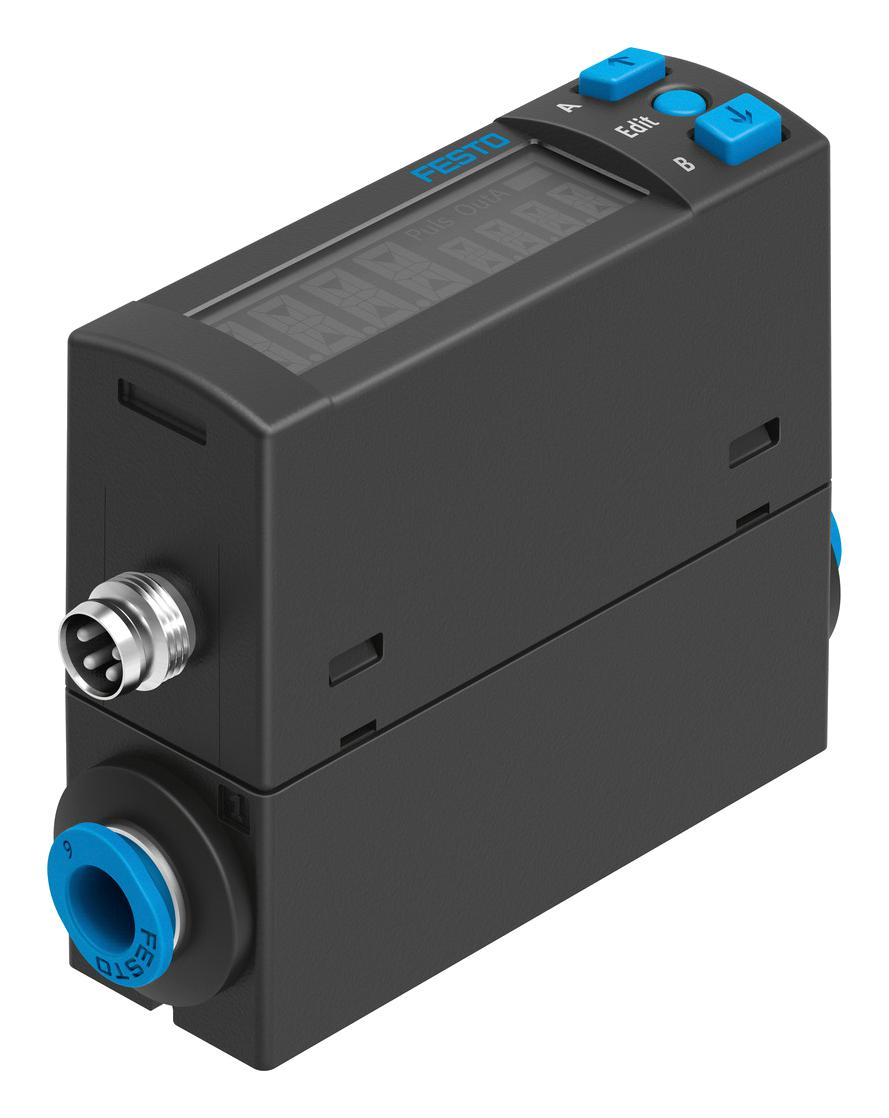
\includegraphics[scale = 0.1]{assets/figures/Festo_debitmetre.jpg}
                  \caption{Débitmètre Festo}
              \end{subfigure}
              \begin{subfigure}{0.5\textwidth}
                  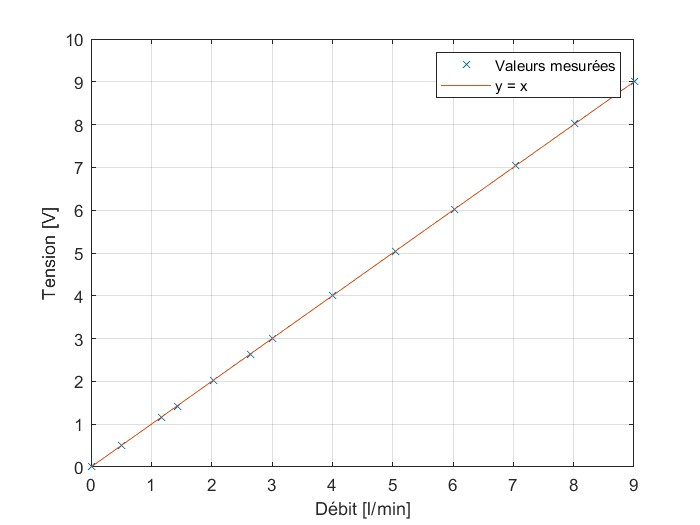
\includegraphics[scale = 0.4]{assets/figures/Calibration_maison.jpg}
                  \caption{Sortie analogique - Tension en fonction du débit}
                  \label{fig:calibration}
              \end{subfigure}
              \caption{Débitmètre de référence}
          \end{figure}
          
          Sur la figure \ref{fig:calibration}, nous pouvons observer la tension mesurée en fonction d'un certain débit d'air. Les paramètres utilisés
          pour cette calibration sont les suivants :
          \begin{itemize}
              \item Sortie analogique en tension sur une plage de 0 V à 10 V
              \item Full Scale allant de 0\% à +100\%
          \end{itemize}
          
          Pour les paramètres donnés, le graphe montre une fonction linéaire qui se rapproche très fortement de la fonction $y = x$ (f$_{mesur\acute{e}}(x) = 1.0004x - 0.0038$).\\
          
          La sortie analogique du débimètre sera également utilisée afin de comparer la sortie du débitmètre de référence et la sortie du capteur 
          \gls{capteur}. \\
          
    \item \textbf{Électrovanne FESTO MHE3-MS1H-3/2G-QS-6-K}\\
          Cette électrovanne fonctionne avec une tension de 24 V.  Elle permet de créer un flux d'air pulsé. Ce flux d'air pulsé alimentera le
          capteur \gls{capteur} à partir d'air comprimé.\\
          Cet appareil possède 3 ports de connexion et 2 commutations différentes (également dit : vanne à 3/2 voies) disposés selon le schéma ci-dessous :
          \begin{figure}[H]
              \centering
              \begin{subfigure}{0.45\textwidth}
                  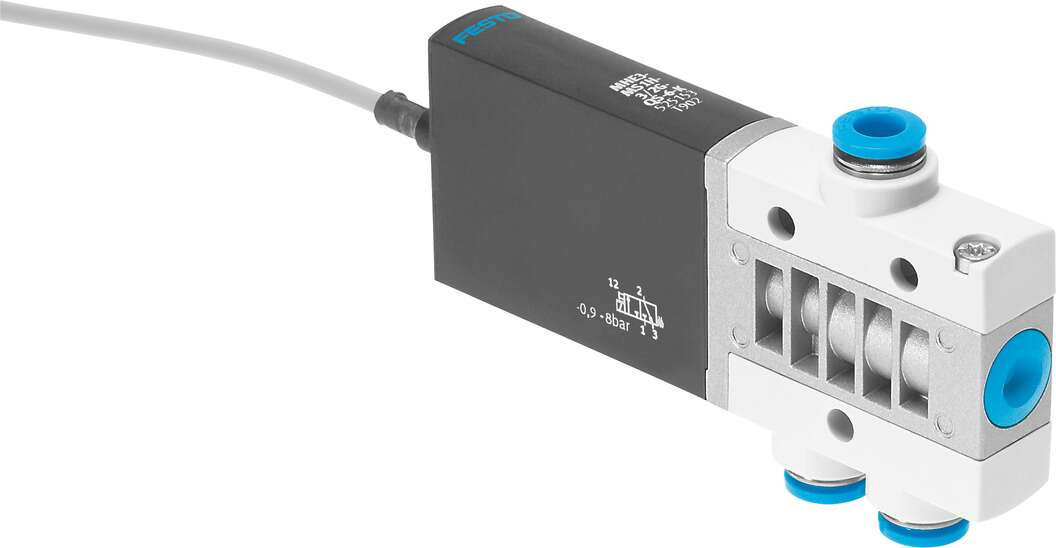
\includegraphics[scale=0.1]{assets/figures/Electrovanne.jpg}
                  \caption{Électrovanne Festo}
              \end{subfigure}
              \begin{subfigure}{0.45\textwidth}
                  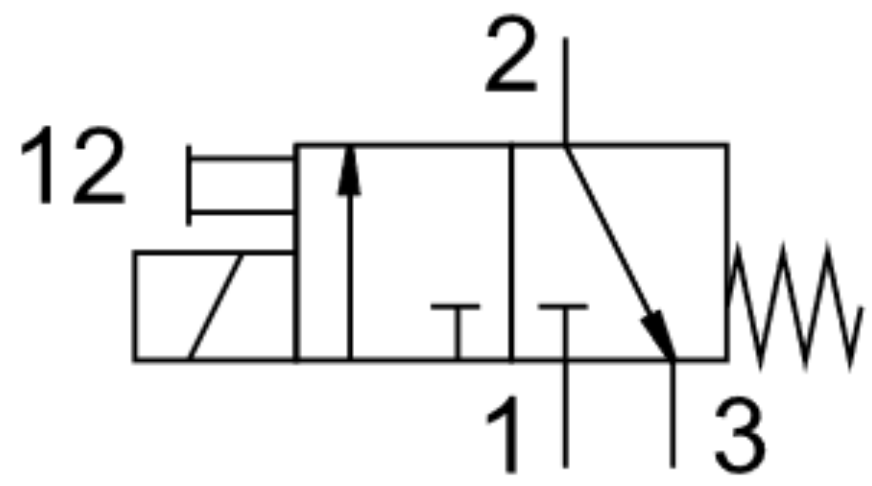
\includegraphics[scale = 0.3]{assets/figures/Electrovanne_InOutput.png}
                  \caption{Schéma d'électrovanne \cite{electrovanne}}
                  \label{fig:electrovanne_InOutput}
              \end{subfigure}
              \caption{Électrovanne}
          \end{figure}
          Les entrées/sorties sont représentées par les numéros 1, 2 et 3. L'électrovanne est représentée par deux carrés accolés (cf. figure
          \ref*{fig:electrovanne_InOutput}). Le carré de gauche montre le système au repos. Le carré de droite représente la deuxième position de
          l'électrovanne, lorsque celle-ci est mise sous tension \cite{electrovanne}.\\
          
          Pour les mesures avec un flux d'air pulsé, l'arrivée d'air comprimé sera connecté à l'entrée numérotée 3 et la sortie de l'électrovanne se fera à 
          la sortie numérotée 2. \\
          Puis une alimentation viendra alimenter l'électrovanne à une certaine fréquence. Ainsi, lorsque l'électrovanne recevra 24 V, elle laissera 
          passer le flux d'air de 3 à 2 et lorsque l'électrovanne sera hors-tension, elle bloquera le flux d'air. \\
          
          Pour les mesures de flux d'air continu, l'entrée numéro 1 sera utilisée à la place de l'entrée numéro 3. Ceci permettra la circulation du 
          flux d'air de manière continue lorsque l'électrovanne est hors-tension. \\
          
    \item \textbf{Transistor \gls{mosfet} IRL540N}\\
          Le \gls{mosfet} (metal-oxide-semiconductor field-effect transistor) est un transistor fonctionnant en tension. Dans notre cas, il va
          être utilisé comme un interrupteur qui va alimenter ou non l'électrovanne. \\
          Le \gls{mosfet} possède trois branches nommées D (drain), G (gate) et S (source). 
          \begin{figure}[H]
              \centering
              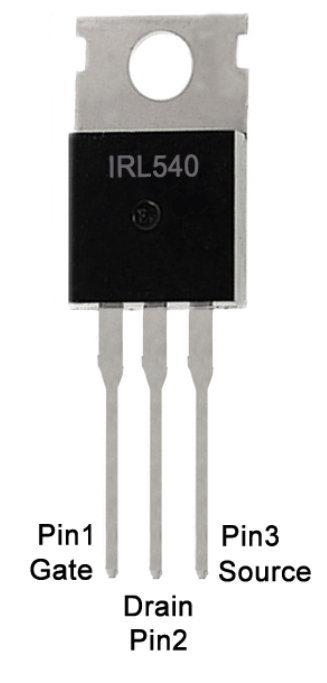
\includegraphics[scale = 0.3]{assets/figures/mosfet_visuel.png}
              \caption{\gls{mosfet}}
              \label{fig:mosfet}
          \end{figure}
          \newpage
    \item \textbf{Arduino Nano}\\
          L'Arduino Nano est un circuit-imprimé (cf. figure \ref{fig:arduino}) qui va également participer à la création du flux d'air pulsé.
          \begin{figure}[H]
              \centering
              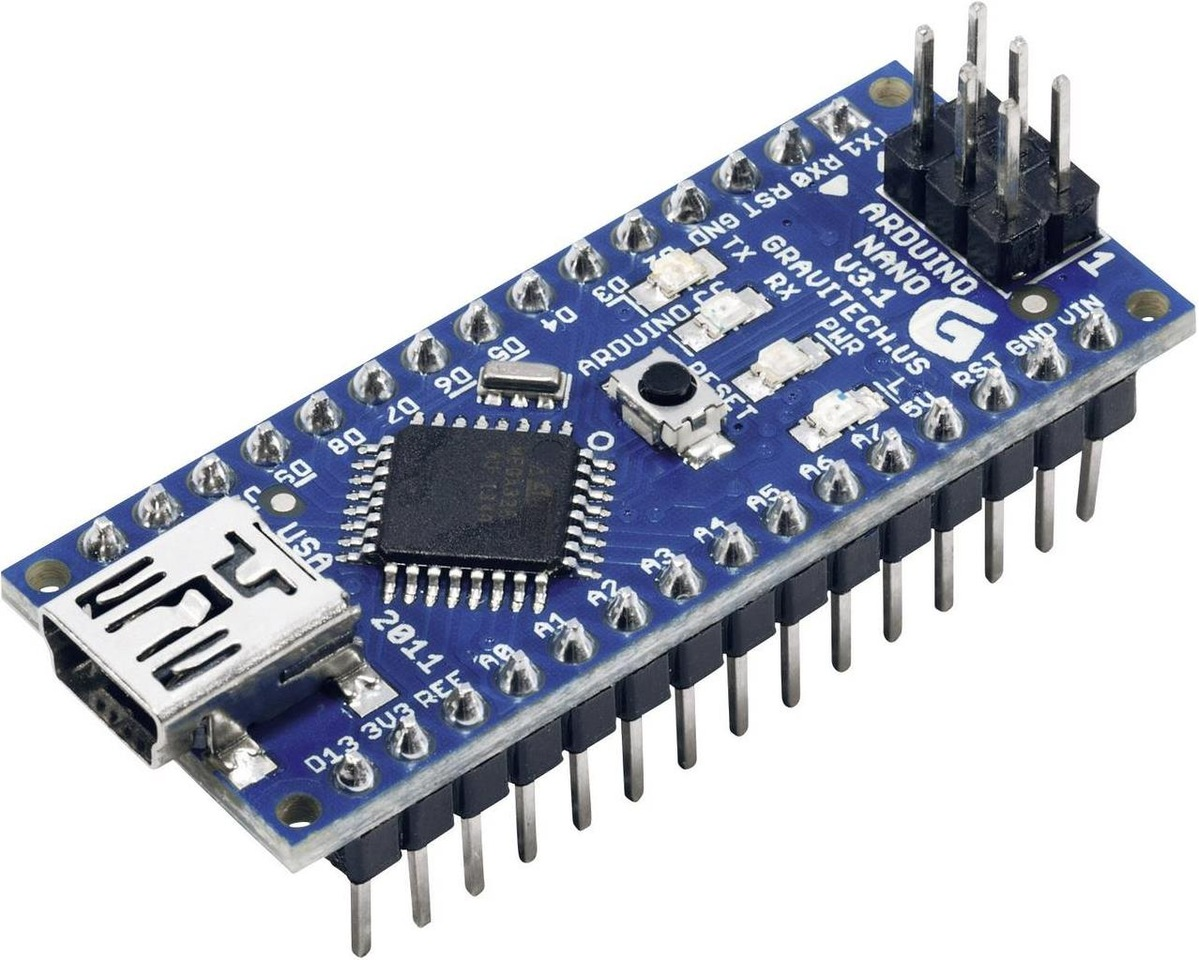
\includegraphics[scale = 0.11]{assets/figures/Arduino-Board-Nano-ATMega328.jpg}
              \caption{Arduino Nano}
              \label{fig:arduino}
          \end{figure}
          C'est grâce à l'arduino que la fréquence du flux d'air sera modulable. En effet, ce composant va contrôler le \gls{mosfet}, qui 
          transmettra ensuite les informations à l'électrovanne.\\
          Le code utilisé afin de créer une sortie en tension par pulsation est fourni en annexe. Il a été réalisé sur le logiciel Arduino IDE.\\
\end{itemize}

Toutes les Datasheets des composants utilisés et achetés se trouvent en annexe. Ces Datasheets contiennent toutes les valeurs et schémas nécessaires
au dimensionnement du banc de test.
\newpage
\section{Modélisation du banc de test}
\subsection{Gestion du flux d'air}
\subsubsection{Flux d'air pulsé}
Une première possibilité est d'amener un flux d'air pulsé sur la membrane. Comme mentionné, ce flux d'air serait contrôlé par une électrovanne et un
transistor MOSFET IRL540N. Ce transistor a été choisi, car il permet d'être contrôlé grâce à un Arduino Nano. En effet, sa tension de seuil
($V_{GS}$) est de 4 V, 5 V ou 10 V. Étant donné que l'Arduino Nano sortira une tension de 5 V, cette valeur sera suffisante pour faire fonctionner
le \gls{mosfet}. La figure \ref{fig:MOSFET} illustre le fonctionnement du flux pulsé avec l'électrovanne, l'Arduino Nano et le \gls{mosfet} et 
ses trois connexions (D, G et S). 
\begin{figure}[H]
    \centering
    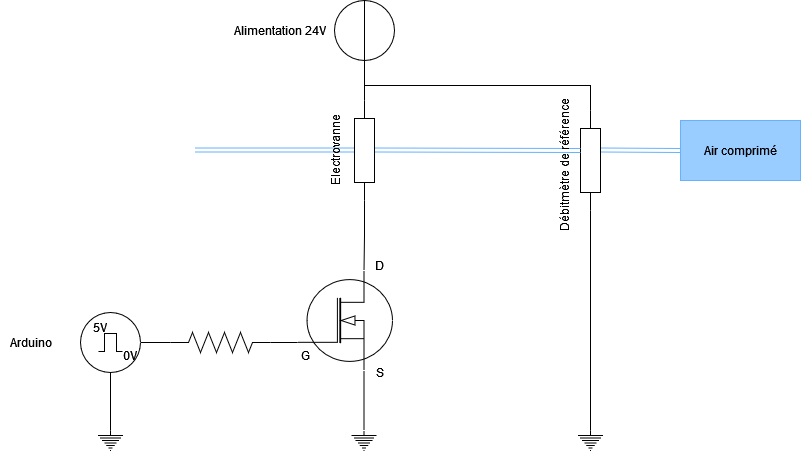
\includegraphics[scale=0.6]{assets/figures/MOSFET.png}
    \caption{Schéma d'utilisation du \gls{mosfet}}
    \label{fig:MOSFET}
\end{figure}
Un contrôle de la chaleur dégagée par le transistor (par effet Joule) est utile afin de décider si un dissipateur thermique est nécessaire. Ce calcul se fait
de la manière suivante :\\

D'abord, calculons la chaleur dégagée (puissance par effet Joule) :

\[I_{electrovanne} = \frac{P_{electrovanne}}{U} = \frac{6.5}{24} \cong 0.27 \text{ A} \]
\[P_{effetJoule} = R_{DS}\cdot I^2\]
Avec :\\
$R_{DS}$ (résistance entre les jonctions D et S du \gls{mosfet}) = 0.053 $\Omega$

Ainsi :
\begin{equation}
    P_{effetJoule} = 0.053\cdot 0.27^2 \cong 3.86 \text{ mW}
\end{equation}

Les différentes valeurs de résistances, puissances, etc. se trouvent dans la datasheet du MOSFET qui se trouve en annexe. \\

Puis, nous pouvons calculer la puissance maximum dissipée par le \gls{mosfet} :
\[P_{max\,dissip\acute{e}e} = \frac{max(T_j) - T_A}{R_{\theta JA}} = \frac{175-25}{62}\cong 2.42 \text{ W}\]
Avec :\\
$T_j$ = température de jonction [\textdegree C]\\
$T_A$ = température ambiante [\textdegree C]\\
$R_{\theta JA}$ = résistance thermique, de la température de jonction à ambiante [$\Omega$]

Ainsi, comme $P_{effetJoule} < P_{max\,dissip\acute{e}e}$, un dissipateur thermique n'est pas nécessaire \cite{addohms_mosfets_2014}. \\

Au niveau du fonctionnement du flux pulsé, le transistor est commandé par un Arduino Nano qui alimente le \gls{mosfet} avec 5 V par pulsation 
(par exemple : 1 seconde à 5 V et 1 seconde à 0 V). \\
Lorsque le \gls{mosfet} reçoit 5 V, il s'active et laisse circuler le courant qui permet à l'électrovanne de s'activer et de faire passer le
flux d'air.
\begin{figure}[H]
    \centering
    \begin{subfigure}[b]{0.45\textwidth}
        \hspace{-1.5cm}
        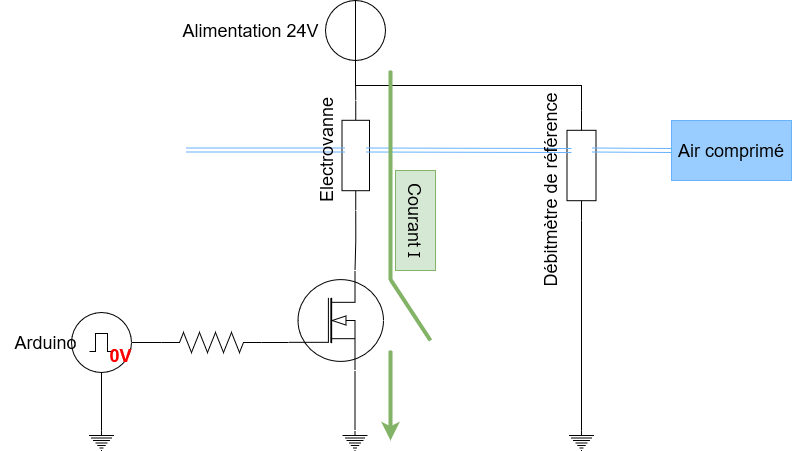
\includegraphics[scale = 0.3]{assets/figures/MOSFET_0V.png}
        \caption{\gls{mosfet} non alimenté}
        \label{fig:MOSFET_0V}
    \end{subfigure}
    \begin{subfigure}[b]{0.45\textwidth}
        \centering
        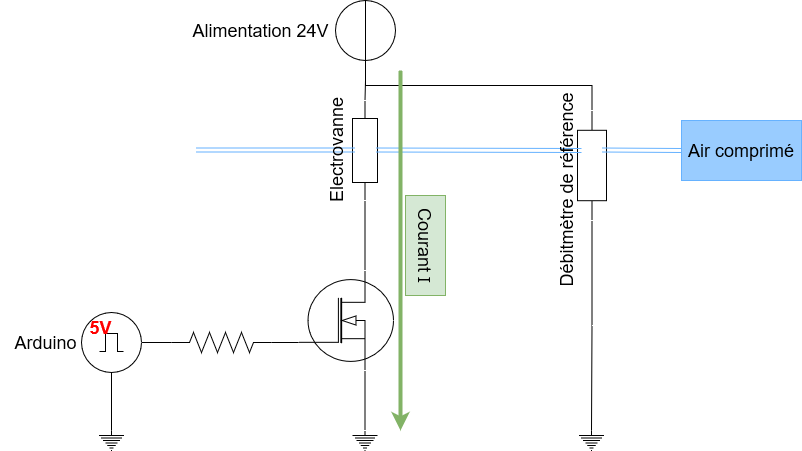
\includegraphics[scale = 0.3]{assets/figures/MOSFET_5V.png}
        \caption{\gls{mosfet} alimenté}
        \label{fig:MOSFET_5V}
    \end{subfigure}
    \caption{Fonctionnement du flux d'air pulsé}
    \label{fig:flux_pulse}
\end{figure}

\subsubsection{Flux d'air continu}
Deux manières permettent d'obtenir un flux d'air continu. \\

Si la tension de 24 V est active, la programmation de l'Arduino peut être modifiée afin d'alimenter le \gls{mosfet} de manière continue. 
Ainsi l'électrovanne sera, elle aussi, sous tension de manière continue. \\

Une autre manière est de dés-alimenter le \gls{mosfet}, et de brancher l'arrivée d'air à l'entrée 1 de l'électrovanne comme expliqué sous la 
figure \ref{fig:electrovanne_InOutput}. 

\subsection{Gestion du corps de chauffe}
\label{chap:corps_de_chauffe}
Le corps de chauffe, constitué d'une fine couche d'or, doit être alimenté avec un certain courant. Ce courant, s'il est trop élevé, va abîmer la
membrane, mais s'il est trop bas, il sera insuffisant pour entraîner une différence de température de part et d'autre du capteur. \\

Les calculs suivant ont donc été effectués afin de déterminer le courant à utiliser pour le corps de chauffe :
\[P_{max} = R\cdot I^2\]
Avec :\\
$P_{parSurface}$ (puissance max par unité de surface) = 100 $\frac{\text{W}}{\text{m}^2}$\\
$R$ (résistance du corps de chauffe) = 75 $\Omega$ (pour l'échantillon D06)\\

La valeur de puissance par unité de surface a été tirée de la puissance maximale utilisée pour les chauffages du marché (chauffage au sol) 
\cite{noauthor_choisir_nodate}.
Elle permet d'avoir un ordre de grandeur pour la valeur de courant à fournir au corps de chauffe.
La surface du corps de chauffe a été approximée à 80 mm$^2$ (2 mm $\cdot$ 40 mm).\\
Ainsi une règle de 3 a été effectuée afin de trouver la valeur de puissance maximale pour le corps de chauffe concerné :
\[P_{max} = 8\cdot 10^{-5}\cdot 100 = 8\cdot 10^{-3} \text{ W}\]
\[I = \sqrt{\frac{P_{max}}{R}} = \sqrt{\frac{8\cdot 10^{-3}}{75}} \cong 10.33\text{ mA}\]
Plusieurs tests ont été alors effectué dans une plage de 10 mA à 20 mA. Ces tests ont donné un courant maximum à 15 mA. Au-delà, la membrane
est abîmée (couche d'or rongée).\\

Ces calculs ont été faits afin d'obtenir une estimation de l'ordre de grandeur du courant à utiliser. Ils ne prennent pas en compte l'épaisseur 
de la couche conductrice. C'est pour cette raison qu'une vérification réelle (avec le corps de chauffe physique) a été effectuée. Une épaisseur 
plus conséquente d'or permet certainement la circulation d'une valeur courant plus élevé. 

\subsubsection{Corps de chauffe continu}
Afin de chauffer le corps de chauffe de manière continue, une alimentation de laboratoire peut être utilisée. Pour ce projet, une double 
alimentation est utilisée. Un côté de l'alimentation sort un courant maximal de 15 mA pour le corps de chauffe et l'autre côté sort 24 V pour 
les autres composants. 

\subsubsection{Corps de chauffe pulsé}
\label{chap:corps_chauffe_pulse}
Une manière de tester les capteurs \gls{capteur} serait de faire pulser le corps de chauffe et d'amener un flux d'air constant. \\
Cela signifie qu'il faut alimenter le corps de chauffe un certain temps, puis couper l'alimentation. Ceci peut se faire, comme pour l'arrivée
d'air pulsé, par un relais, un transistor tel le \gls{mosfet} ou un générateur de fonction. \\

Pour ce projet, un générateur de fonction a été utilisé afin de simplifier le processus. Ce générateur de fonction sort un signal carré
d'une certaine tension (dépendante de la résistance du corps de chauffe) avec un offset permettant d'avoir un front descendant autour des
0 V. La tension est choisie en fonction de la résistance du corps de chauffe et du courant souhaité (ici 15 mA, cf. chapitre 
\ref{chap:corps_de_chauffe}). En utilisant la loi d'Ohm $U = R\cdot I$, la tension est facilement calculée.

\subsubsection{Schémas blocs du banc de test}
La figure \ref{fig:schema_cables} illustre les différents composants du banc de test ainsi que le câblage électrique.
\begin{figure}[H]
    \centering
    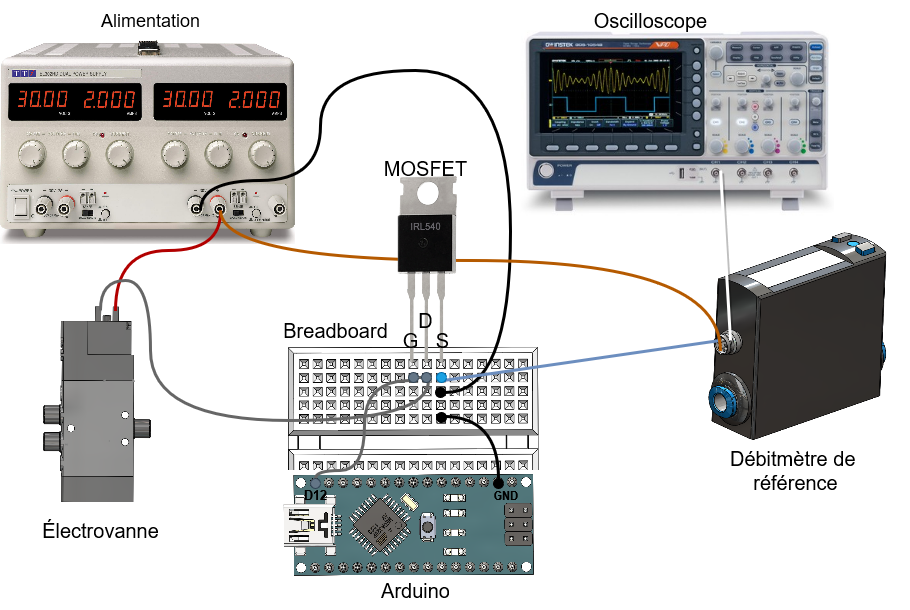
\includegraphics[scale = 0.35]{assets/figures/cablage_electrique.png}
    \caption{Schéma bloc du banc de test}
    \label{fig:schema_cables}
\end{figure}

Une alimentation de laboratoire est utilisée pour les 24 V requit par l'électrovanne et le débitmètre de référence. Puis, une platine d'expérimentation 
(breadboard) est consacrée à la connexion du \gls{mosfet} et de l'Arduino. \\

Le capteur, quant à lui, est situé dans un circuit relativement déconnecté du système illustré par la figure \ref{fig:schema_cables}. 
\begin{figure}[H]
    \centering
    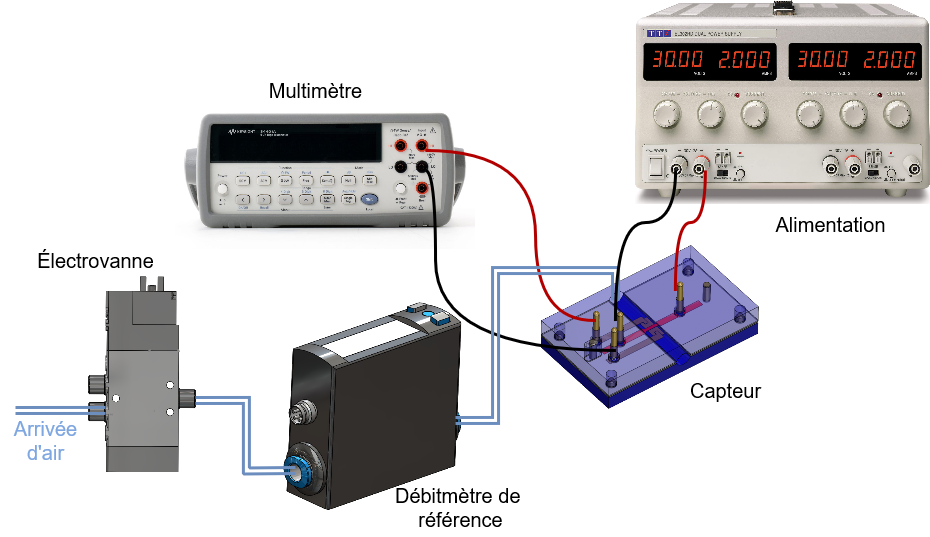
\includegraphics[scale=0.35]{assets/figures/Raccord_air.png}
    \caption{Schéma bloc des connexions autour du capteur}
    \label{fig:circuit_capteur}
\end{figure}
Le capteur \gls{capteur} est relié au débitmètre de référence et à l'électrovanne par les tuyaux d'air comprimé. Il est ensuite connecté soit directement au 
multimètre soit à l'oscilloscope via l'amplificateur. La figure \ref{fig:circuit_capteur} illustre le cas du multimètre. \\

Le corps de chauffe du capteur peut être alimenté soit par une alimentation (corps de chauffe continu), soit par un générateur de fonction (corps 
de chauffe cadencé). La figure \ref{fig:circuit_capteur} montre le cas du corps de chauffe continu. 

\subsection{Conception 3D et réelle du banc de test}
\begin{figure}[H]
    \centering
    \begin{subfigure}{0.45\textwidth}
        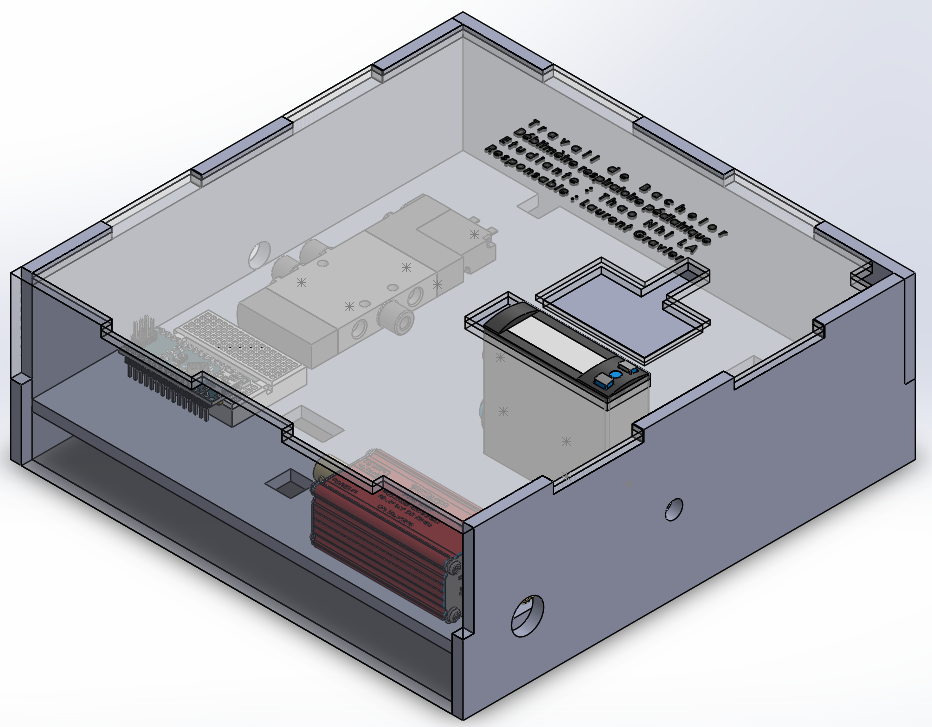
\includegraphics[scale = 0.4]{assets/figures/Banc_de_test.png}
        \caption{Conception 3D du banc de test}
        \label{fig:3D_banc_test}
    \end{subfigure}
    \hspace{1cm}
    \begin{subfigure}{0.45\textwidth}
        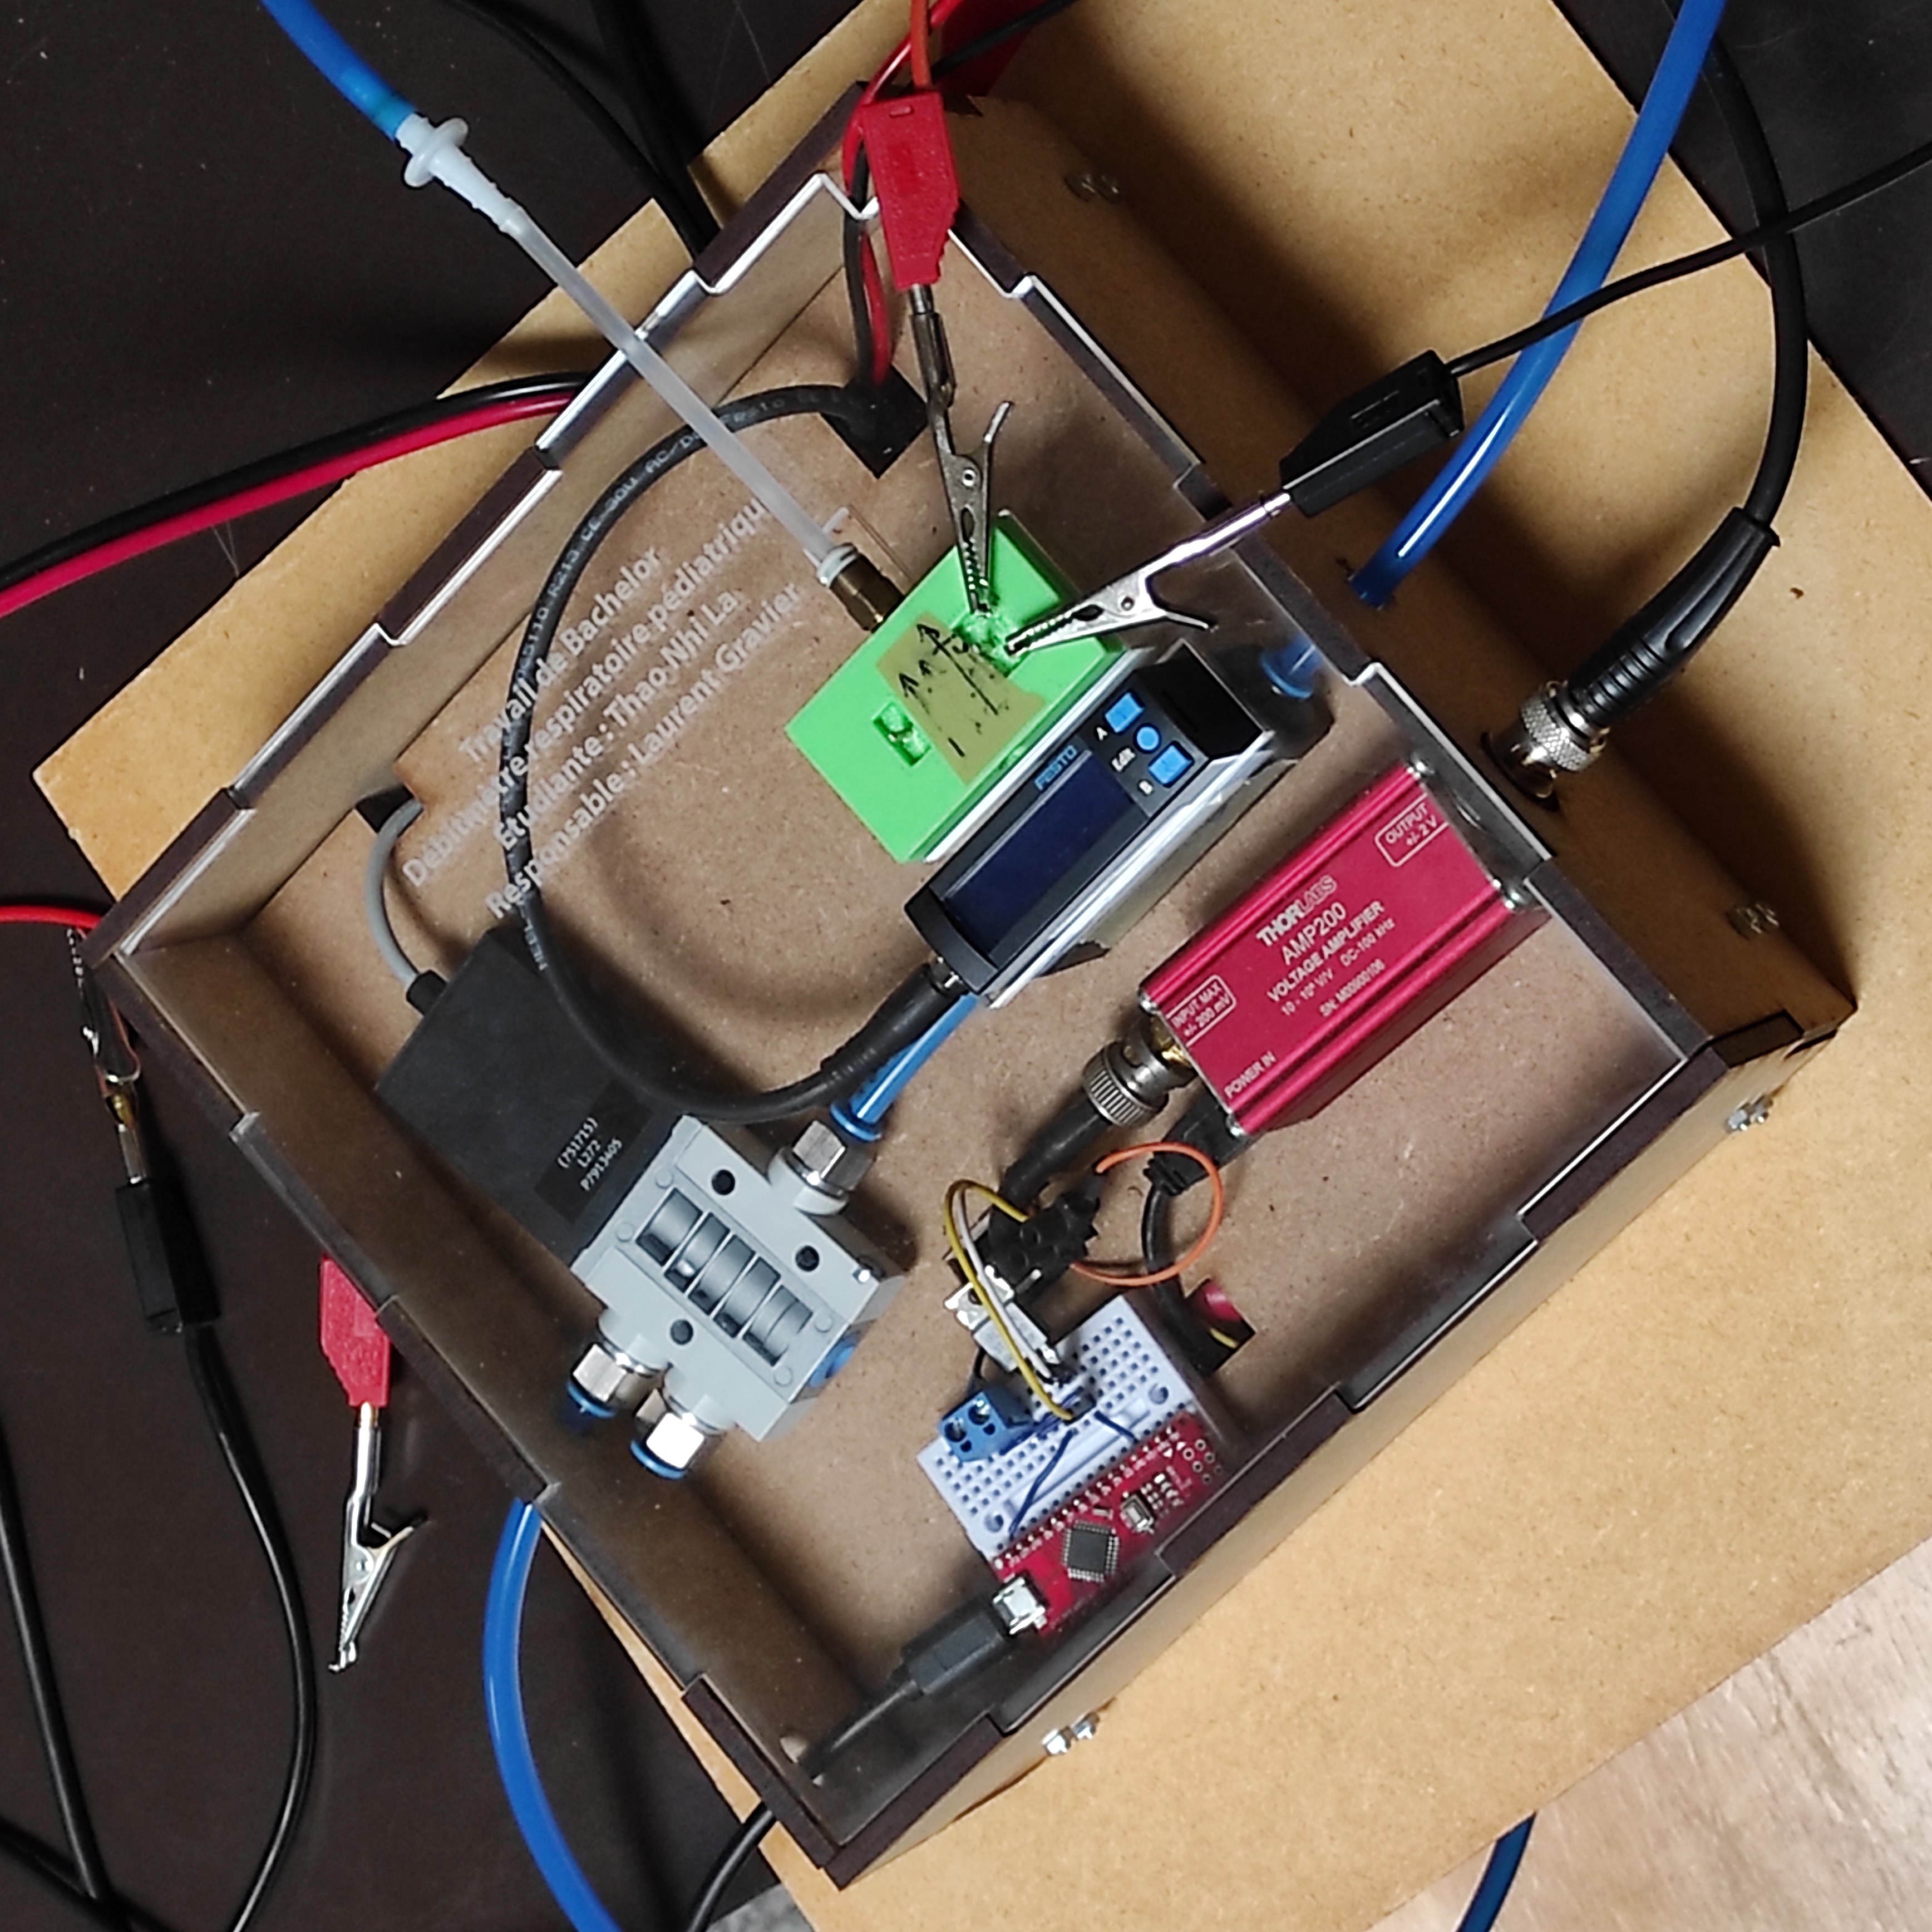
\includegraphics[scale = 0.05, angle = -90]{assets/figures/Banc_de_test_real.png}
        \caption{Réalisation du banc de test}
        \label{fig:banc_test_reel}
    \end{subfigure}
    \caption{Banc de test}
    \label{fig:banc_test}
\end{figure}

La figure \ref{fig:banc_test_reel} montre le banc de test réalisé. Les murs du boîtier sont en MDF et le couvercle est en plexiglas. Un double 
fond (visible sur la figure \ref{fig:3D_banc_test}) a été mis en place afin d'y ranger les câbles. 

\newpage
\section{Mise en place et paramétrage du banc de test}
\begin{enumerate}
    \item Brancher les différents composants du banc de test selon le schéma \ref{fig:schema_cables} et \ref{fig:circuit_capteur}.
    \item L'alimentation 24 V est réglée avec une tension maximale à 24 V et un courant maximal autour des 1 A.
    \item Le générateur de fonction, s'il est utilisé, est paramétré avec un signal carré d'amplitude ($V_{pp}$) égale à la moitié de la tension souhaitée
          (cf. chapitre \ref{chap:corps_chauffe_pulse}) et avec un décalage (offset) égal à la moitié de l'amplitude citée précédemment. 
    \item L'entrée de l'oscilloscope pour le débitmètre de référence peut être paramétré avec une division en temps à 5 s ou 10 s et une division
          en tension à 2 V. 
    \item Le programme LabView était déjà écrit et est réutilisé pour ce projet. Il se trouve en annexe. \\
          Le paramètre encadré en rouge sur l'annexe est important, car il permet d'ajuster la vitesse d'acquisition et la gamme souhaitée. 
          
          %\item Brancher l'alimentation 24 V au banc de test :
          %\begin{itemize}
          %    \item Connecter le pôle positif de l'alimentation à une des broches de l'électrovanne
          %    \item Connecter le pôle négatif de l'alimentation à la broche S du \gls{mosfet} par le Jumper Wire blanc (il s'agit de la connexion à la terre)
          %\end{itemize}
          
          %\item Connecter le débitmètre de référence à l'alimentation :
          %\begin{itemize}
          %    \item Connecter le câble marron du débitmètre au pôle positif de l'alimentation (par exemple, grâce à un câble sortant de l'alimentation
          %          avec une pince crocodile au bout, lier la broche de l'électrovanne et le fil marron du débitmètre)
          %    \item Le câble bleu du débitmètre doit être lié à la broche S du \gls{mosfet} par le biais du bornier à vis sur la Breadboard
          %\end{itemize}
          
          
          %\item Brancher le deuxième brin de l'électrovanne à la broche D du \gls{mosfet} par le bornier à vis\\
          
          %\item Brancher l'amplificateur à une alimentation secteur\\
          
          %\item Brancher l'Arduino Nano à un ordinateur et lancer le programme\\
          
    \item Placer le capteur :
          \begin{itemize}
              \item Connecter le corps de chauffe. Les deux pointes ressorts concernées par le corps de chauffe doivent
                    être connectées soit à l'alimentation de laboratoire fournissant maximum 15 mA, soit au générateur de fonction. 
                    Les pointes ressorts pour le corps de chauffe sont représentées en jaune sur la figure \ref{fig:pointes_ressorts_chauffe}.
                    \begin{figure}[H]
                        \centering
                        \begin{subfigure}[b]{0.45\textwidth}
                            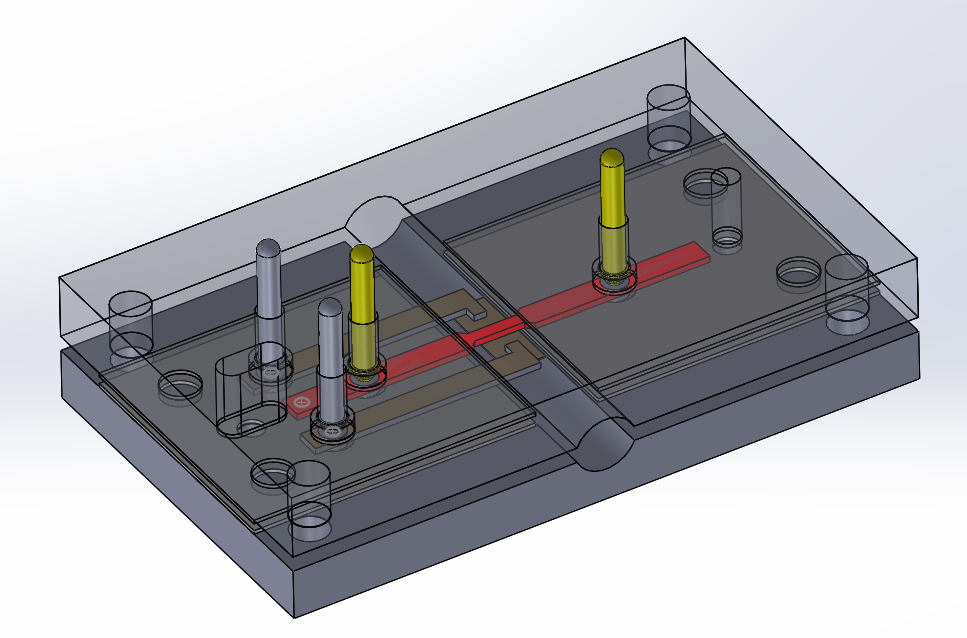
\includegraphics[scale = 0.3]{assets/figures/pointes_ressorts_chauffe.png}
                        \end{subfigure}
                        \begin{subfigure}{0.45\textwidth}
                            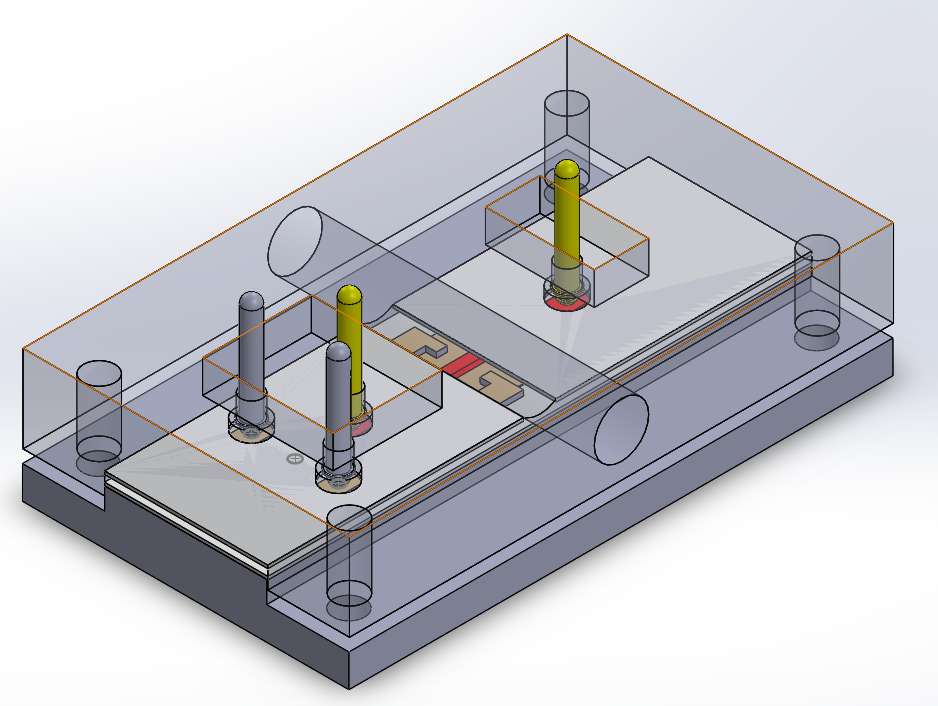
\includegraphics[scale = 0.3]{assets/figures/pointes_ressorts_chauffe_design5.png}
                        \end{subfigure}
                        \caption{Pointes ressorts du corps de chauffe}
                        \label{fig:pointes_ressorts_chauffe}
                    \end{figure}
          \end{itemize}
          
    \item Sortie avec amplificateur : Connecter les deux pointes ressorts restantes à l'amplificateur grâce aux câbles nommés "Amplificateur
          $\leftrightarrow$ Capteur"\\
          
    \item Sortie directe sur LabView : Connecter directement les deux pointes ressorts restantes à l'appareil de mesure utilisé (multimètre
          connecté au programme LabView)
\end{enumerate}

\section{Vérification du banc de test}
Lors des premiers tests, aucun signal n'était visible sur l'oscilloscope. Ceci peut être dû à différentes raisons :
\begin{itemize}
    \item Un mauvais contact avec les pointes ressorts\\
          
    \item La puissance du corps de chauffe n'est pas suffisante\\
          
    \item L'échantillon (capteur \gls{capteur}) est défectueux\\
\end{itemize}

Afin de vérifier quels paramètres entraînent un mauvais résultat, une première décision a été de tester le \gls{capteur} ouvert (sans son support,
en utilisant seulement la membrane).
Des pinces plates viennent faire le contact électrique directement sur les couches d'or afin de mesurer la tension y circulant.
\begin{figure}[H]
    \centering
    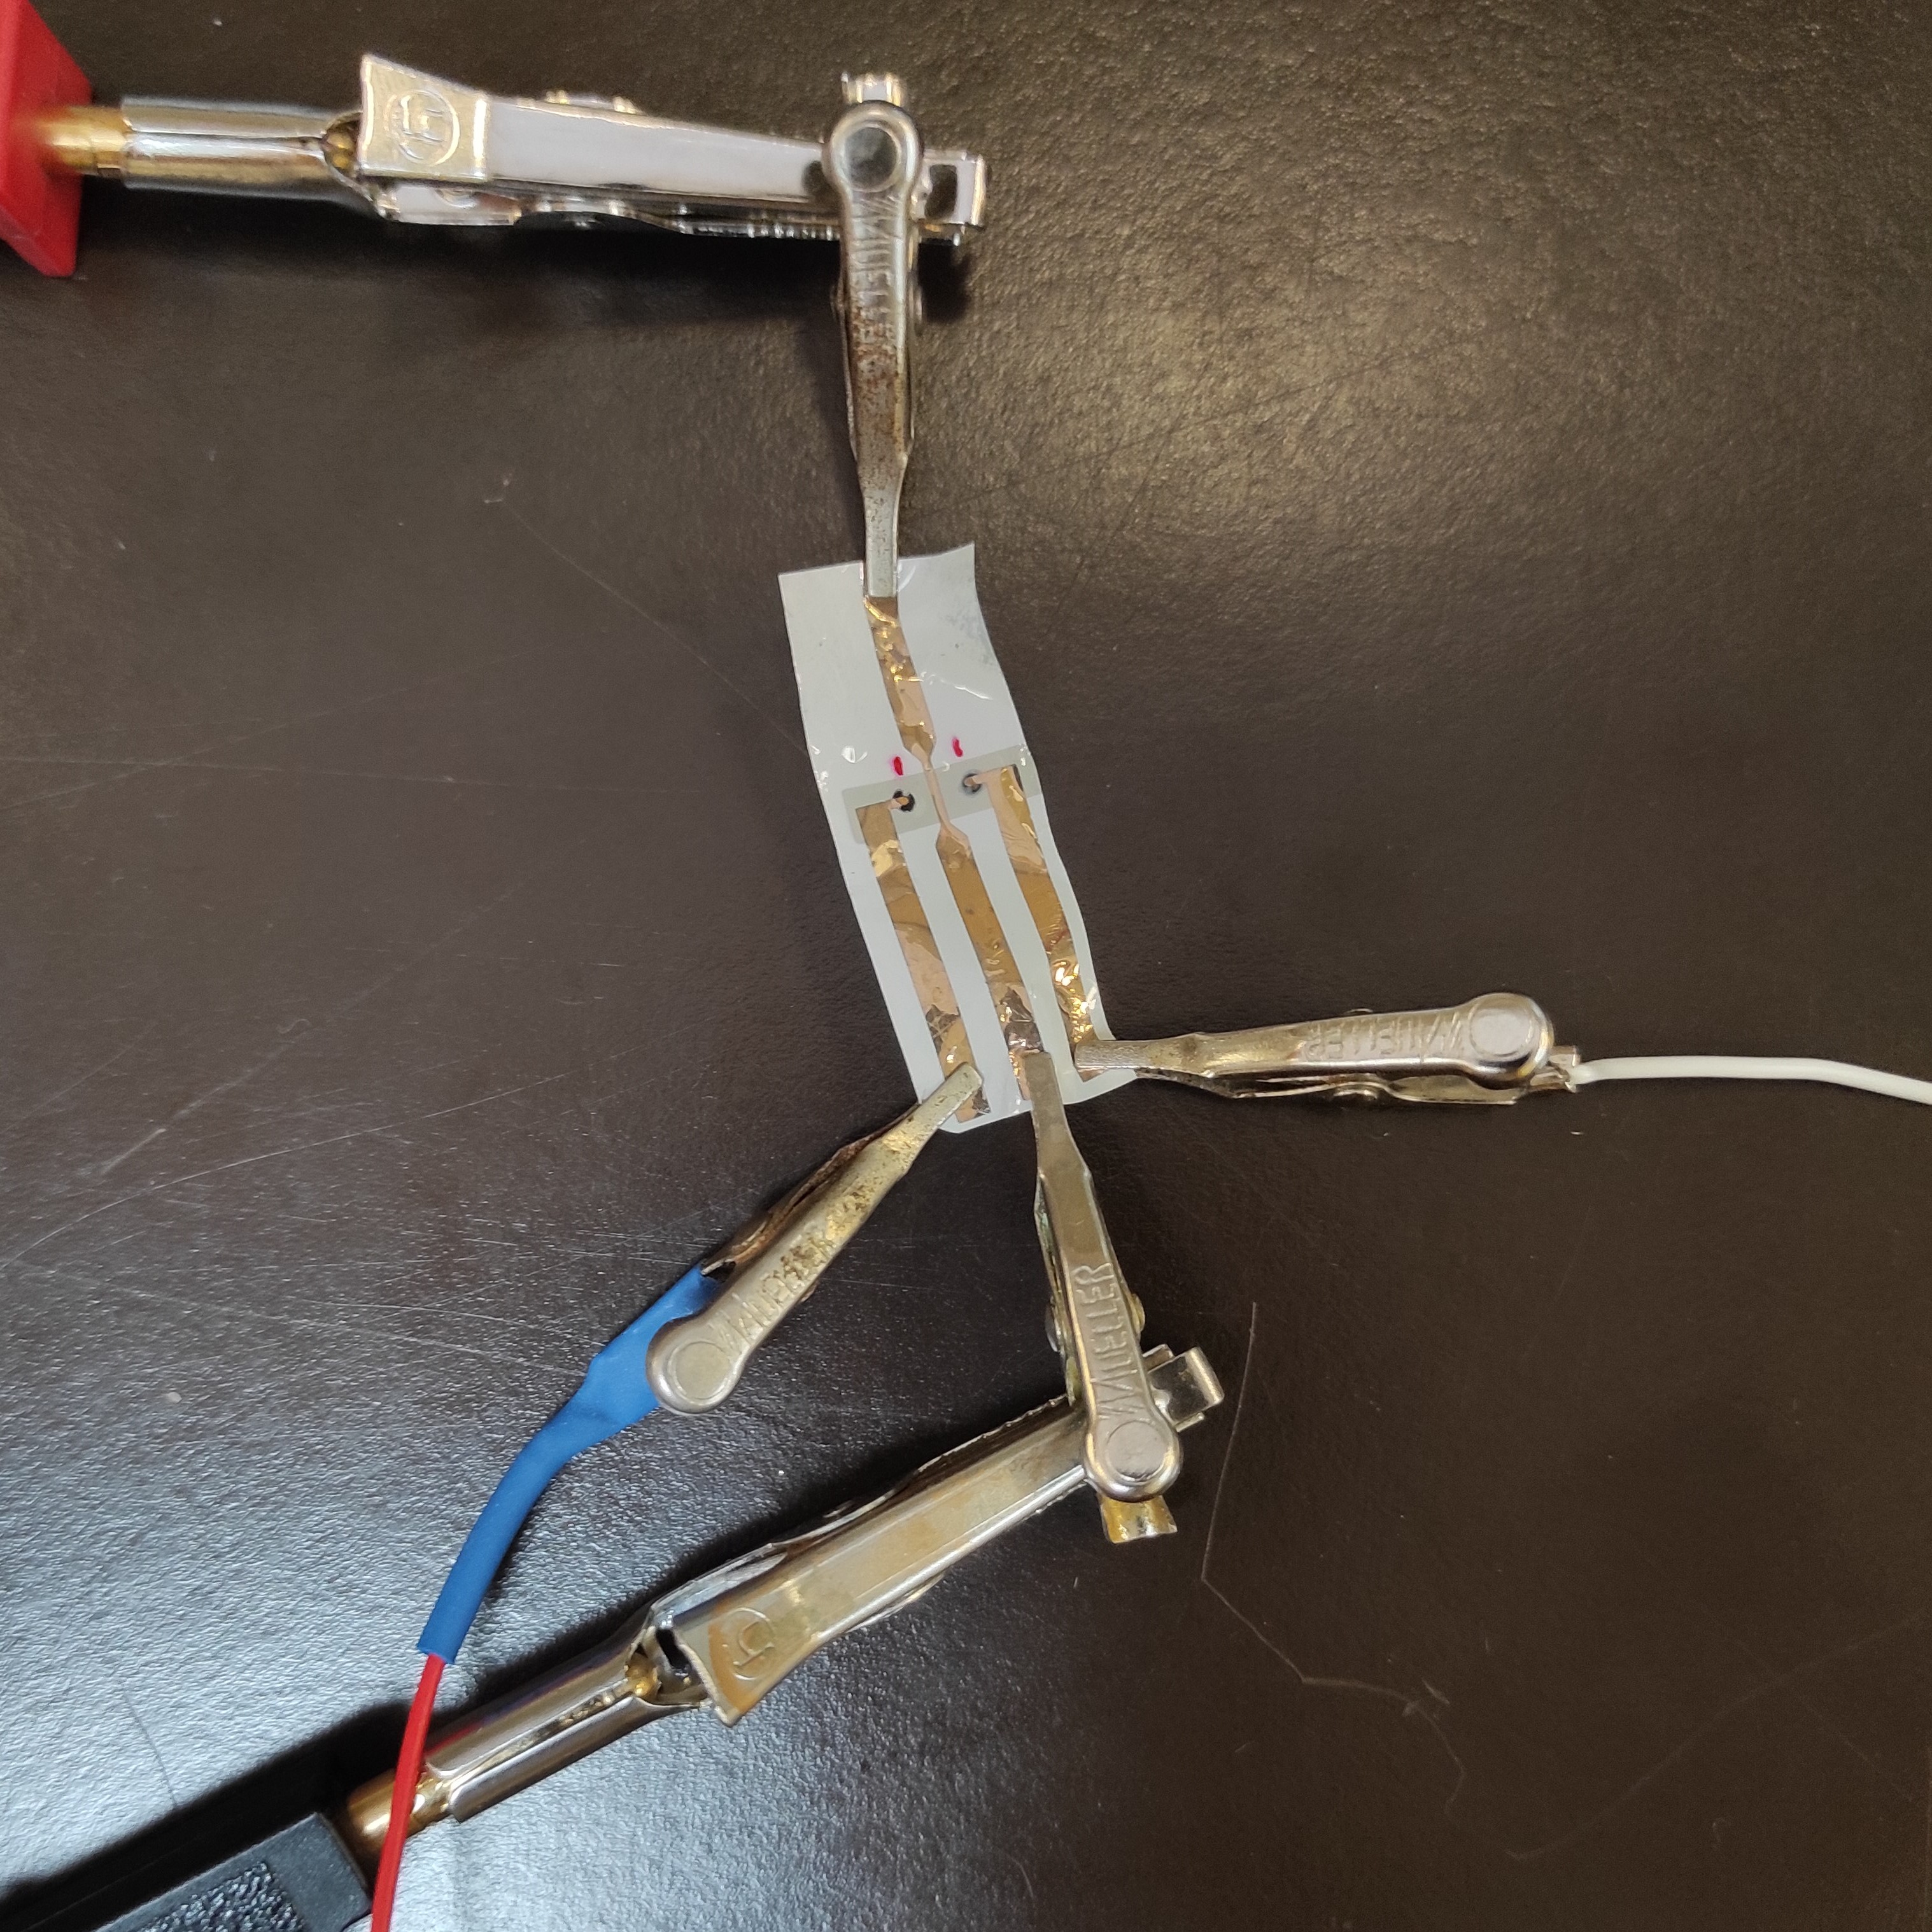
\includegraphics[scale = 0.05]{assets/figures/CapteurOuvert.jpg}
    \caption{Tests sur capteur ouvert}
    \label{fig:capteurOuvert}
\end{figure}
Cette installation ne communiquait pas non plus de résultat concluant (tension oscillant autour des 0 V). \\

Le corps de chauffe a donc été mis en question. Une alternative à ce corps de chauffe a été de venir toucher la pince plate d'un côté du
capteur afin d'engendrer une différence de température entre les deux parties en "L". Ceci a bel et bien entraîné une différence de
température et donc, une tension. Cependant, cette dernière provient de la différence de température entre l'or (sur la membrane) et le métal
de la pince plate. Or, l'objectif est de générer une différence de température entre l'or et le tellure de Bismuth présent dans les électrodépositions. 
En effet, ce couple de matériaux possède un coefficient Seebeck plus avantageux que le métal de la pince et l'or. \\

Ainsi, afin de chauffer une des deux parties électrodéposées, une court tube a été utilisé. Un flux d'air chaud a été soufflé directement sur cette
partie afin de créer un gradient de température, mais à nouveau, aucun résultat n'a été observé. Cela signifie que la jonction avec le tellure
de bismuth est probablement pathologique.\\

Il était tout de même nécessaire et intéressant de vérifier si le banc de test fonctionnait de manière appropriée. Pour cela, un autre capteur
a été utilisé afin de vérifier la fonctionnalité du banc de test. \\
Le capteur utilisé est un capteur infrarouge par nanotechnologie qui traduit un certain rayonnement électromagnétique en tension. Ainsi lorsque l'on souffle
dessus, un changement dans l'environnement, et plus précisément dans la température ambiante, aura lieu. Ce flux d'air impacte donc
les rayonnements thermiques qui, eux, sont étroitement liés, entre autres, aux rayonnements infrarouges. C'est donc pour cette raison qu'à
l'oscilloscope, une fluctuation sur la tension se dessine.
\begin{figure}[H]
    \centering
    \begin{subfigure}[b]{0.45\textwidth}
        \hspace{-1 cm}
        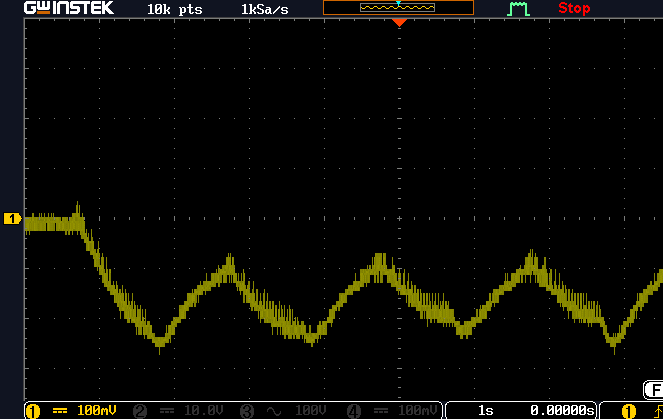
\includegraphics[scale = 0.45]{assets/figures/CapteurIR_1s_1s.PNG}
        \caption{Air pulsé pendant 1 s puis repos pendant 1 s}
        \label{fig:1s1s}
    \end{subfigure}
    \begin{subfigure}[b]{0.45\textwidth}
        \centering
        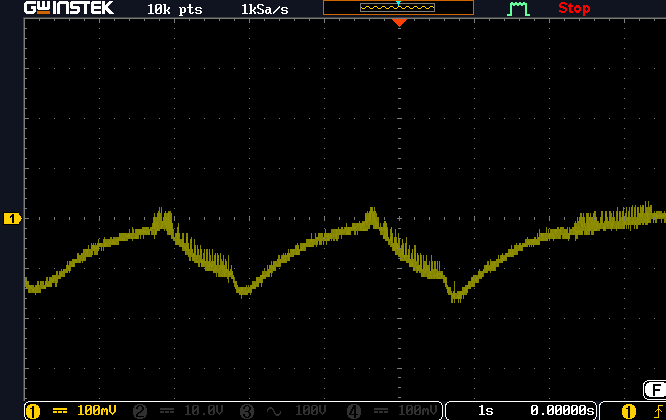
\includegraphics[scale = 0.45]{assets/figures/1_8s_repos.PNG}
        \caption{Air pulsé pendant 1 s puis repos pendant 1.8 s}
        \label{fig:1_8s}
    \end{subfigure}
    \caption{Résultats avec capteur infrarouge}
    \label{fig:capteurIR}
\end{figure}

Les figures ci-dessus (\ref{fig:capteurIR}), montrent que le banc de test et plus précisément, le système de flux d'air pulsé accompagné de
la sortie à l'oscilloscope (en passant par l'amplificateur) fonctionne bien. En effet, sur les figures \ref*{fig:1s1s} et \ref*{fig:1_8s}
les différentes pulsations sont bien visibles.\\

Sur la figure \ref{fig:1s1s}, la récupération du capteur est plus longue que le temps de repos. C'est pourquoi le temps de repos a été allongé
et fixé à 1.8 s (figure \ref*{fig:1_8s}). Ceci permet au capteur de se remettre à zéro et permet aussi de contrôler que la fréquence est bien
modulable. \\

Une autre partie du banc de test intéressante à étudier est l'amplificateur. En effet, lors des premiers essais du banc de test, la sortie de 
l'amplificateur montrait un bruit conséquent régulier. Quelques tests sur ce composant ont donc été réalisés. \\
Par exemple, le facteur d'amplification a été vérifié. Le programme LabView a donc été utilisé afin de mesurer, dans un
premier temps, la réponse du capteur \gls{infrarouge} sans amplificateur, puis, dans un second temps, la réponse avec amplificateur. Ceci nous
permet de calculer le facteur d'amplification réel. Cette manipulation, présente dans les détails en annexe, a donné un facteur d'amplification 
d'environ 670. Cette valeur paraît loin de l'amplification de 1000 indiquée par les données techniques, mais reste dans un ordre de grandeur 
tout à fait correct. \\
De plus, les imprécisions de calculs et de manipulation ne sont pas négligeables dans cette étape. 

Ces différents tests prouvent que le banc de test semble fonctionner de manière adéquate. L'échantillon est alors certainement le facteur engendrant de
mauvais résultats. 

\subsection{Hypothèses concernant l'échantillon pathologique}
\label{chap:hypotheses_echantillon_patho}
Afin de détecter où se situe le problème, les différents paramètres du capteur \gls{capteur} ont été remis en question :
\begin{itemize}
    \item \textbf{Matériau thermoélectrique (ThEl)}\\
          La solution de Tellure de Bismuth est peut-être impure. Une nouvelle solution a été alors refaite.
          
    \item \textbf{Distance des pistes d'or du capteur au corps de chauffe}\\
          La distance entre le corps de chauffe et les piste d'or peut être à revoir, car trop proches les unes des autres, la chaleur du corps
          de chauffe risque de se transmettre aux deux extrémités du capteur. De ce fait, la même température sera mesurable en tout point du
          capteur, n'engendrant donc aucune différence de température entre la partie droite et la partie gauche du capteur \gls{capteur}, et donc aucune
          tension ne sera mesurable.\\
          
    \item \textbf{Épaisseur de la membrane} \\
          Plus la membrane est épaisse, plus la couche d'or de court-circuit sera éloignée des couches d'or en "L". Cela assurerait que la piste 
          de court-circuit n'est pas atteinte par le corps de chauffe. Ceci est important pour des raisons similaires au premier paramètre cité. 
          Un transfert de chaleur faible (voir inexistant) par le biais du court-circuit du capteur \gls{capteur} est souhaitable. \\
          
          L'objectif est alors de faire des capteurs en PI25005 (Kepton) et de les comparer grâce au banc de test aux échantillons en GTTP ou VCTP.
          Ceci permettra de vérifier si l'épaisseur de la membrane est un paramètre important.\\
          
    \item \textbf{Position de la piste de court-circuit}\\
          Afin de s'assurer que le corps de chauffe transmette un minimum de chaleur au deux extrémités du capteur, il est également possible de 
          placer la couche d'or de court-circuit plus distante aux électrodépositions.\\
          
    \item \textbf{Diamètre du via}\\
          Lors de l'électrodéposition, un joint en caoutchouc percé au centre d'un diamètre de 0.3 mm, 0.5 mm ou 1 mm (appelé diamètre du via) permet de concentrer
          l'électrodéposition dans un diamètre contrôlé. Cependant, si le diamètre du via est trop faible, l'électrodéposition peut avoir du mal à
          se produire (phénomènes de bulles, électrodéposition non-régulière, etc.)\\
          Il sera intéressant de produire des échantillons avec un diamètre de via le plus grand possible. 
\end{itemize}

\chapter{Mesures}
\section{Mesures intermédiaires sur le capteur}
\label{chap:mesures}
\subsection{Vérification du corps de chauffe}
Avant toute chose, afin de pouvoir suivre tous les paramètres et le fonctionnement de notre système, une caméra thermique a été utilisée
pour observer le comportement du corps de chauffe

\begin{figure}[H]
    \begin{subfigure}[b]{0.3\textwidth}
        \hspace{-1 cm}
        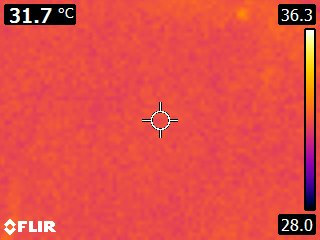
\includegraphics[scale = 0.5]{assets/figures/thermique_sans_chauffe.jpg}
        \caption{Image thermique du capteur - Corps de chauffe éteint}
    \end{subfigure}
    \begin{subfigure}[b]{0.3\textwidth}
        \centering
        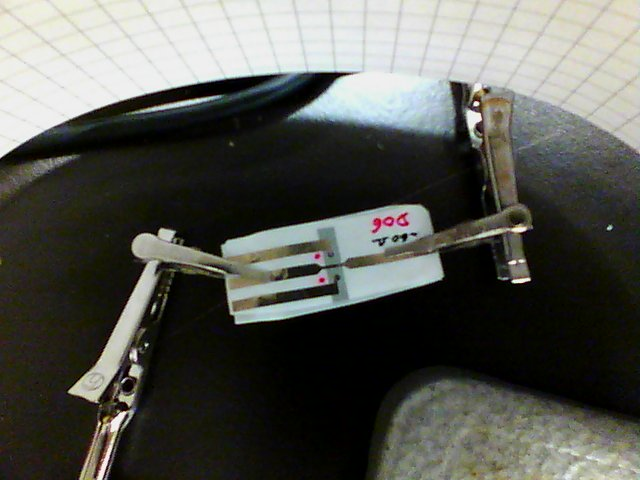
\includegraphics[scale = 0.23]{assets/figures/visuel_avec_chauffe.jpg}
        \caption{Image numérique}
    \end{subfigure}
    \begin{subfigure}[b]{0.4\textwidth}
        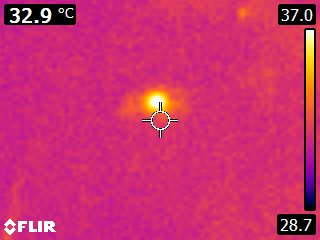
\includegraphics[scale = 0.5]{assets/figures/thermique_avec_chauffe.jpg}
        \caption{Image thermique du capteur - Corps de chauffe allumé}
    \end{subfigure}
    \caption{Résultats de la caméra thermique}
    \label{fig:cameraThermique}
\end{figure}

Il faut savoir que les pistes d'or réfléchissent énormément. Il est donc difficile d'obtenir un résultat parfait. Une première astuce a été de
dessiner au stylo un point noir sur les pistes à mesurer. Ainsi, les problèmes de réflexions seraient amoindris. Malheureusement cette astuce n'a
pas été suffisante. \\

Une autre mesure a alors été faite dans des conditions moins lumineuses (après le coucher du soleil). La figure \ref*{fig:cameraThermique},
montre que le corps de chauffe possède une température avoisinant les 37\textdegree. \\

Un second type de mesure permettant de comprendre chaque partie du \gls{capteur} a été effectuée. Celle-ci concerne la résistance du corps de
chauffe.
\begin{table}[H]
    \begin{center}
        \begin{tabular}{|c|c|c|}
            \hline
            Échantillon n\textdegree & Résistance directe [$\Omega$] & Résistance pointes ressort [$\Omega$] \\
            \hline
            D04                      & 28.28                         & 27.58                                 \\
            \hline
            D06                      & 81.85                         & 72.34                                 \\
            \hline
        \end{tabular}
        \caption{Résistance à travers les pointes ressort}
        \label{tab:resistancePointeRessort}
    \end{center}
\end{table}
Sur le tableau \ref*{tab:resistancePointeRessort}, une différence entre la resistance mesurée directement sur la piste d'or du corps de
chauffe (résistance appelée Résistance directe) et la résistance à travers les pointes ressort est visible. Ceci peut être dû au fait que
les pointes ressort ont également une petite résistance qui vient alors changer la résistance totale du corps de chauffe. Cependant, il faut
également prendre en compte le fait que la résistance change suivant la position de la mesure. En effet, une mesure faite aux extrémités de
la piste d'or sera différente d'une mesure effectuée sur le centre de la piste d'or.

\subsection{Hypothèses concernant l'échantillon défectueux}
Afin de détecter où se situe le problème, les différents paramètres du capteur \gls{capteur} ont été remis en question :
\begin{itemize}
    \item \textbf{Matériau thermoélectrique (ThEl)}\\
          La solution de Tellure de Bismuth est peut-être impure. Une nouvelle solution a été alors refaite.

    \item \textbf{Distance des pistes d'or du capteur au corps de chauffe}\\
          La distance entre le corps de chauffe et les piste d'or peut être importante, car trop proches, les unes des autres, la chaleur du corps
          de chauffe risque de se transmettre aux deux extrémités du capteur. De ce fait, la même température sera mesurable en tout point du
          capteur, engendrant donc aucune différence de température entre la partie droite et la partie gauche du \gls{capteur}, et donc aucune
          tension ne sera mesurable.\\

    \item \textbf{Epaisseur de la membrane} \\
          Plus la membrane est épaisse, plus la couche d'or de court-circuit sera éloignée. Cela permettrait à la source de chaleur d'être concentrée
          à un endroit spécifique. Ceci est important pour des raisons similaires au premier paramètre cité. Un transfert de chaleur faible (voir
          inexistant) entre les deux extrémités du \gls{capteur} est souhaitable (c'est la différence de température qui va engendrer une tension
          mesurable). \\

          Dans le stock de matière de membranes se trouvent les choix suivant :
          \begin{itemize}
              \item GTTP 6-10$\mu$m d'épaisseur
              \item VCTP 6-10$\mu$m d'épaisseur
              \item PI25005 25$\mu$m d'épaisseur
          \end{itemize}
          L'objectif sera alors de faire des capteurs en PI25005 (Kepton) et de les comparer grâce au banc de test aux échantillon en GTTP ou VCTP.
          Ceci permettra de affirmer ou désaffirmer l'hypothèse.\\

    \item \textbf{Diamètre du via}\\
          Lors de l'électrodéposition, un joint en caoutchouc percé au centre d'un diamètre de 0.3mm, 0.5mm ou 1mm (appelé diammètre du via) permet de concentrer
          l'électrodéposition aux endroits souhaités. Cependant, si le diamètre du via est trop faible, l'électrodéposition peut avoir du mal à
          se produire (phénomènes de bulles, électrodéposition non-régulière, etc.)\\

    \item \textbf{Position de la piste de court-circuit}\\
          Afin de s'assurer que le corps de chauffe de transmet pas la chaleur au deux extrémités du capteur, il serait possible de placer la couche
          d'or de court-circuit plus distantes aux électrodépositions
\end{itemize}

\begin{comment}
\section{Résultats concluants}
Avec une nouvelle solution de Tellure de Bismuth et deux nouvelles électrodépositions sur une membrane de GTTP, de nouvelles mesures ont été
effectuées. Ces mesures nous ont montré que le capteur fonctionnait. En effet, une réponse a été mesurée.
\begin{table}[H]
    \begin{center}
        \begin{tabular}{|c|c|}
            \hline
            Condition du capteur                                   & Tension mesurée à travers l'amplificateur \\
            \hline
            Corps de chauffe désactivé et arrivée d'air désactivée & 5 mV                                      \\
            \hline
            Corps de chauffe activé et arrivée d'air désactivée    & 0 V                                       \\
            \hline
            Corps de chauffe activé et arrivée d'air activée       & 8 mV                                      \\
            \hline
        \end{tabular}
    \end{center}
\end{table}
Malgré le bruit non-négligeable mesuré à travers l'amplificateur, la tension change suivant les conditions du capteur. Afin de se concentrer
uniquement sur la réponse du capteur, l'amplificateur a été mis de côté pour les futures mesures.
\end{comment}

\section{Procédure de mesures "classiques"}
\begin{enumerate}
    \item Mesure avec un corps de chauffe pulsé\\
    \item Mesure avec un corps de chauffe pulsé et un flux d'air comprimé constant\\
    \item Mesure avec un flux d'air comprimé pulsé et un corps de chauffe constant\\
    \item Mesure sans corps de chauffe et une respiration humaine\\
    \item Mesure avec corps de chauffe constant et respiration humaine
\end{enumerate}

Ces mesures ont été effectuées sur quatre échantillons (quatre types de capteurs) :
\begin{table}[H]
    \centering
    \begin{tabular}{|c|c|c|}
        \hline
        Échantillon & Membrane & Méthode d'électrodéposition \\
        \hline
        D06         & GTTP     & A                           \\
        \hline
        D12         & PI25005  & A                           \\
        \hline
        D13         & PI25005  & B                           \\
        \hline
        D14         & VCTP     & A                           \\
        \hline
    \end{tabular}
\end{table}

Les méthodes d'électrodéposition correspondent à la définition suivante :
\begin{itemize}
    \item Méthode A
          \begin{figure}[H]
              \hspace{-0.5cm}
              \begin{subfigure}{0.45\textwidth}
                  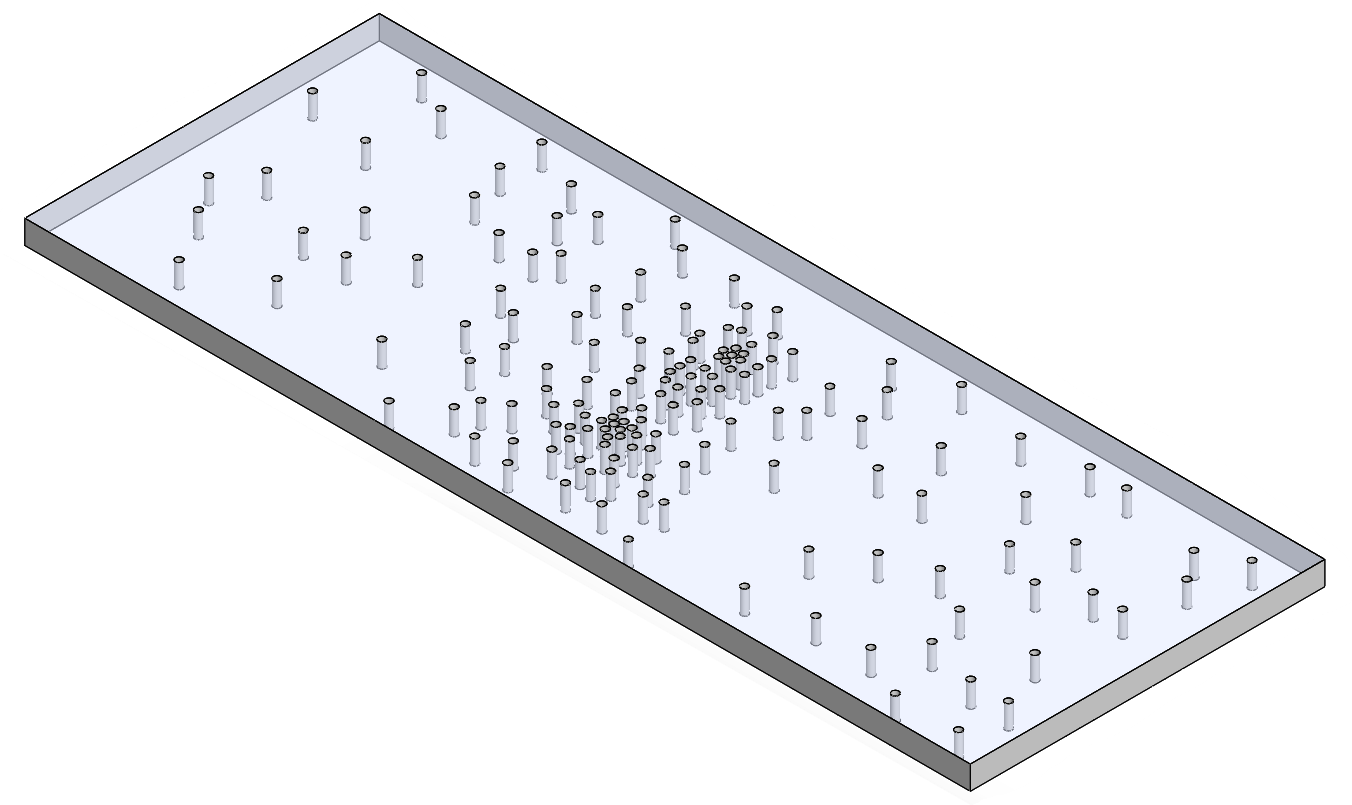
\includegraphics[scale = 0.3]{assets/figures/Membrane_nue.png}
                  \caption{Membrane nanoporeuse}
              \end{subfigure}
              \begin{subfigure}{0.45\textwidth}
                  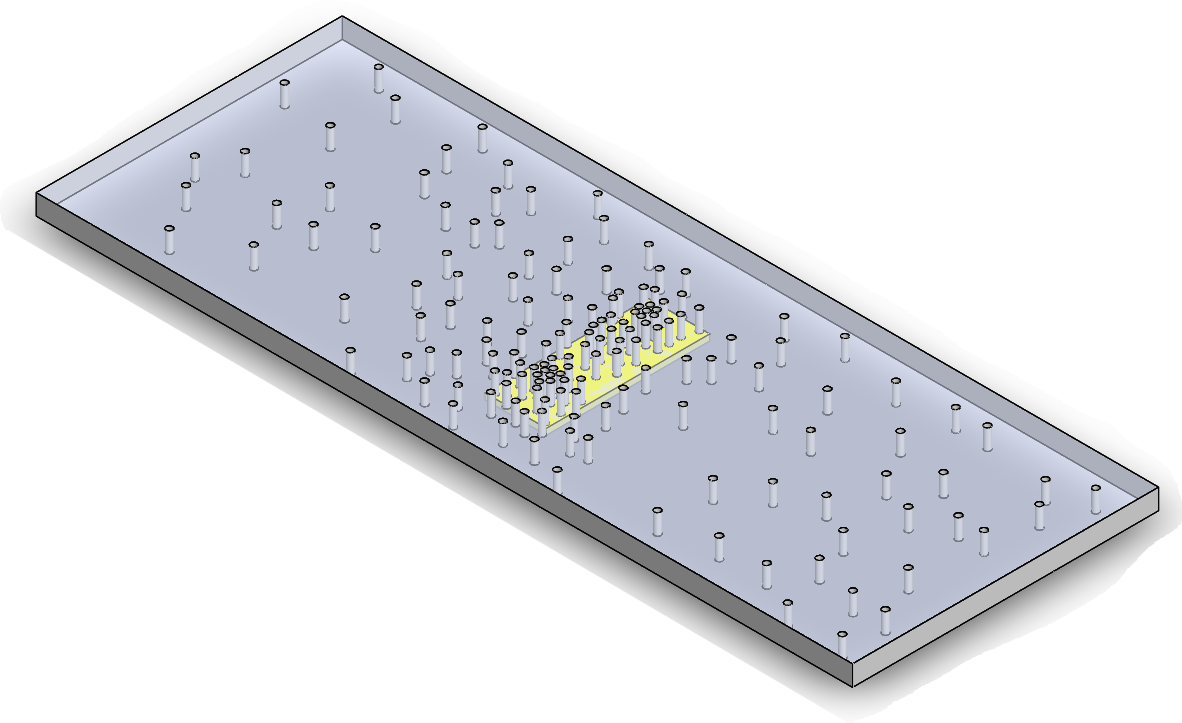
\includegraphics[scale = 0.35]{assets/figures/Court_circuit.png}
                  \caption{Dépôt physique en phase vapeur (PVD) d'or du court-circuit}
              \end{subfigure}
              \newline
              \begin{subfigure}{0.45\textwidth}
                  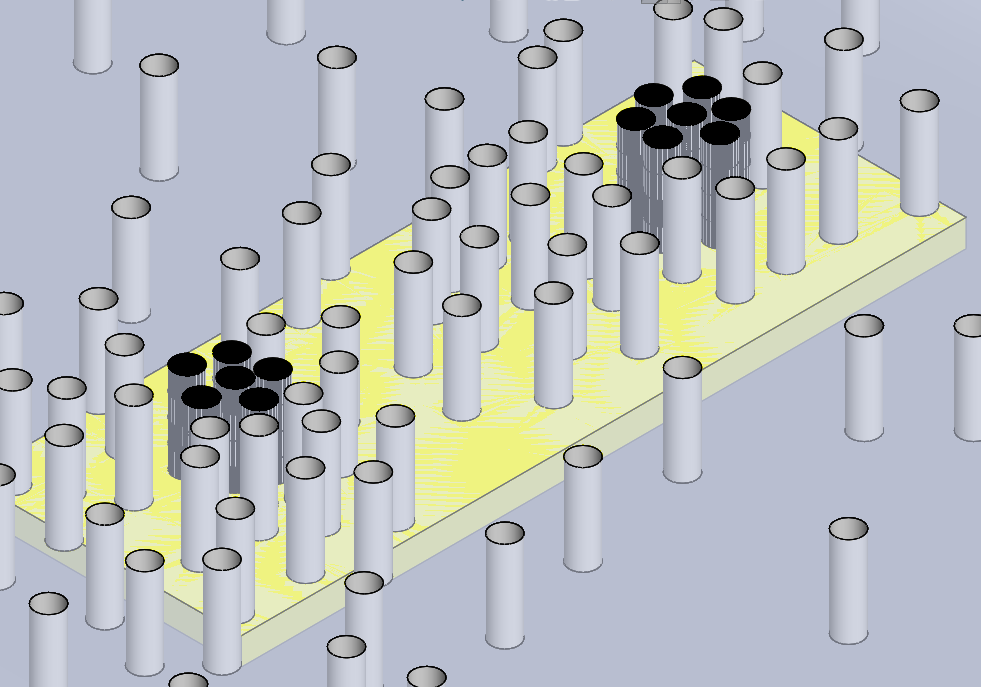
\includegraphics[scale = 0.35]{assets/figures/ED.png}
                  \caption{Électrodépositions effectuées une après l'autre}
              \end{subfigure}
              \begin{subfigure}{0.45\textwidth}
                  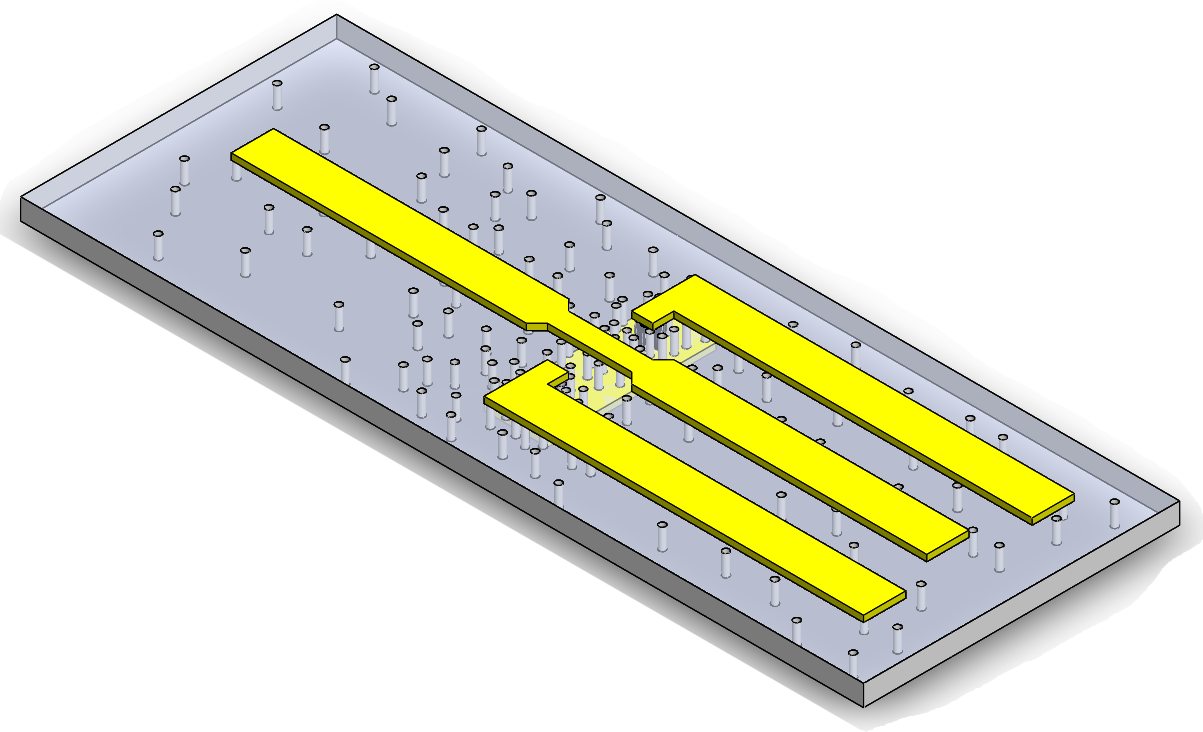
\includegraphics[scale = 0.35]{assets/figures/PVD_L.png}
                  \caption{PVD d'or des branches en L}
              \end{subfigure}
          \end{figure}
    \item Méthode B
          \begin{figure}[H]
              \hspace{-0.5cm}
              \begin{subfigure}{0.45\textwidth}
                  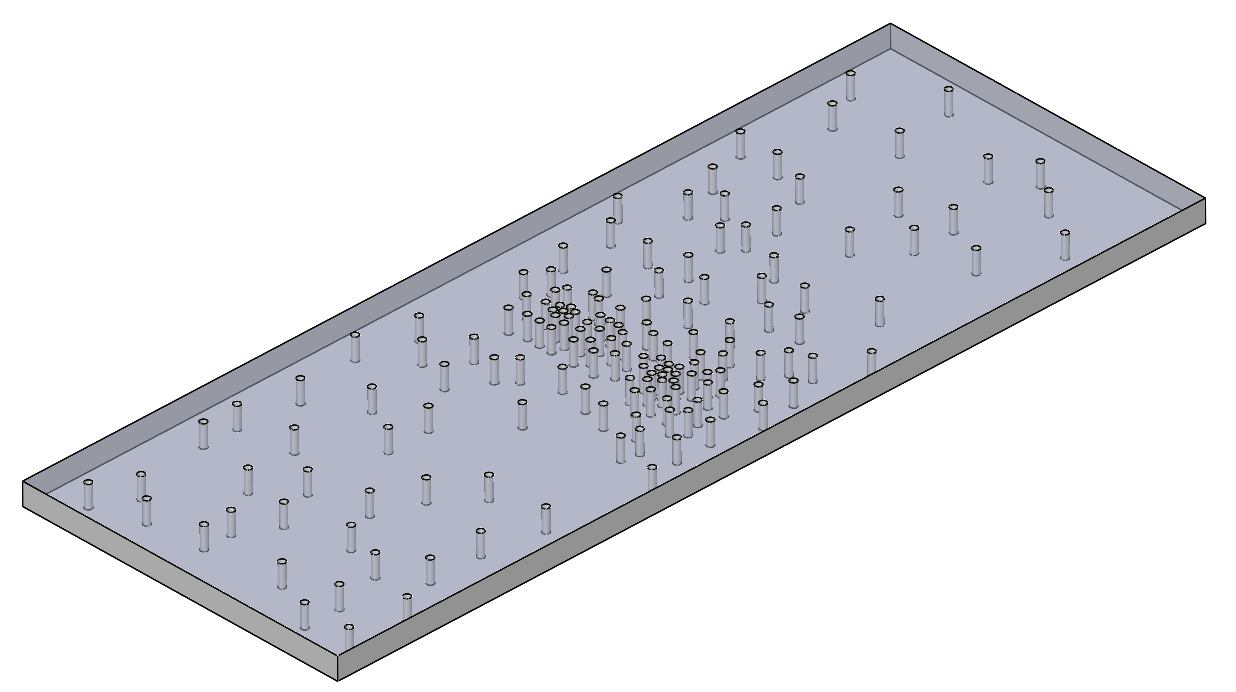
\includegraphics[scale = 0.35]{assets/figures/Membrane_nue_B.png}
                  \caption{Membrane nanoporeuse}
              \end{subfigure}
              \begin{subfigure}{0.45\textwidth}
                  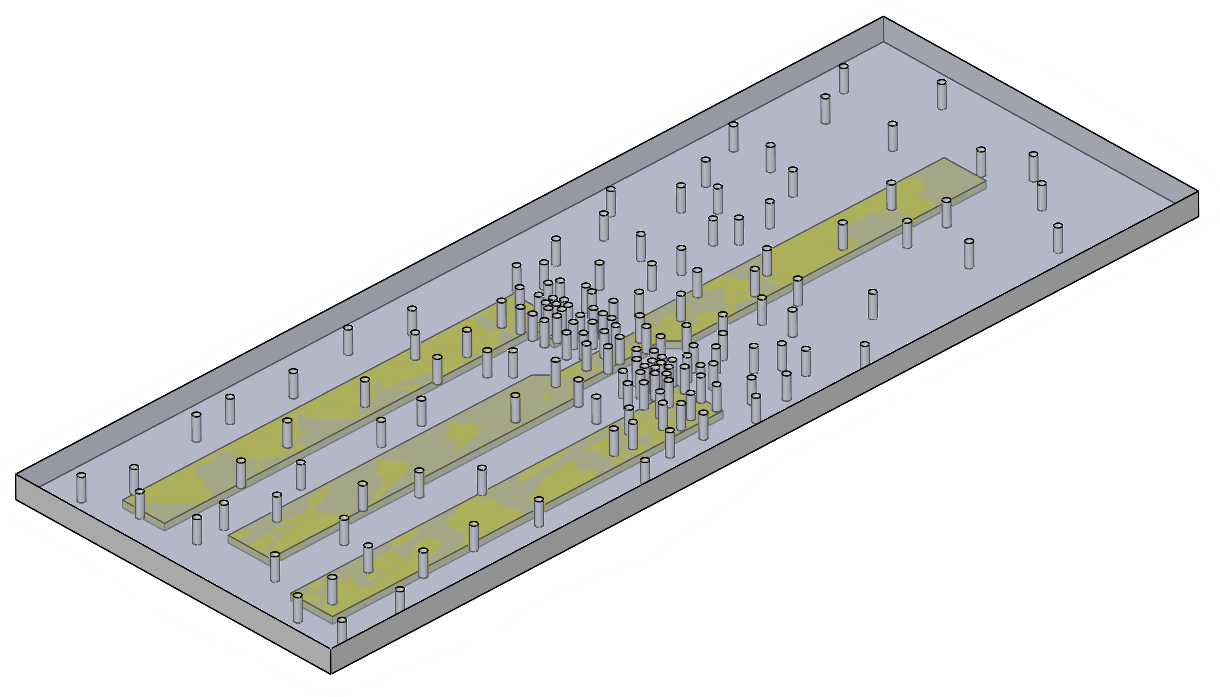
\includegraphics[scale = 0.35]{assets/figures/PVD_L_B.png}
                  \caption{PVD d'or des branches en L}
              \end{subfigure}
              \newline
              \begin{subfigure}{0.45\textwidth}
                  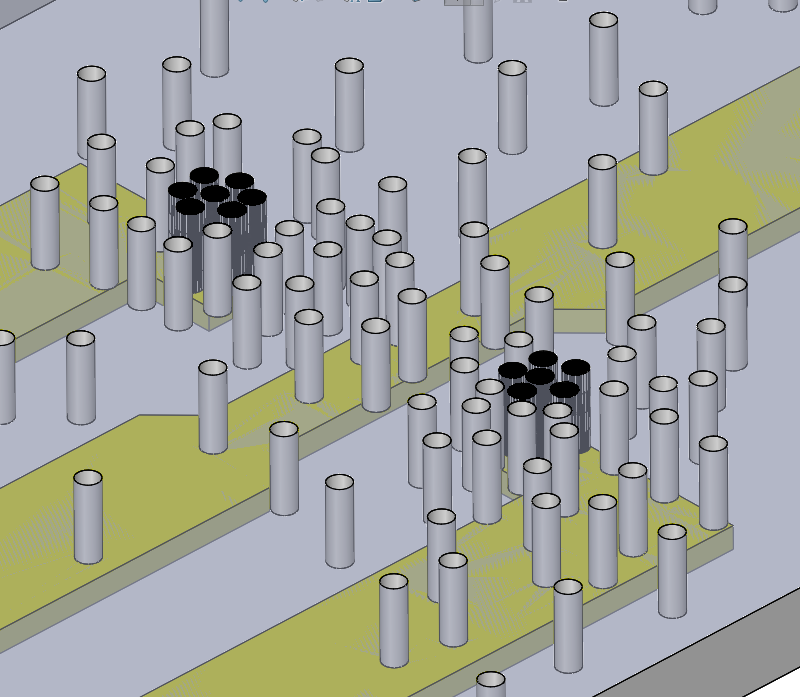
\includegraphics[scale = 0.35]{assets/figures/ED_B.png}
                  \caption{Électrodépositions effectuées une après l'autre}
              \end{subfigure}
              \begin{subfigure}{0.45\textwidth}
                  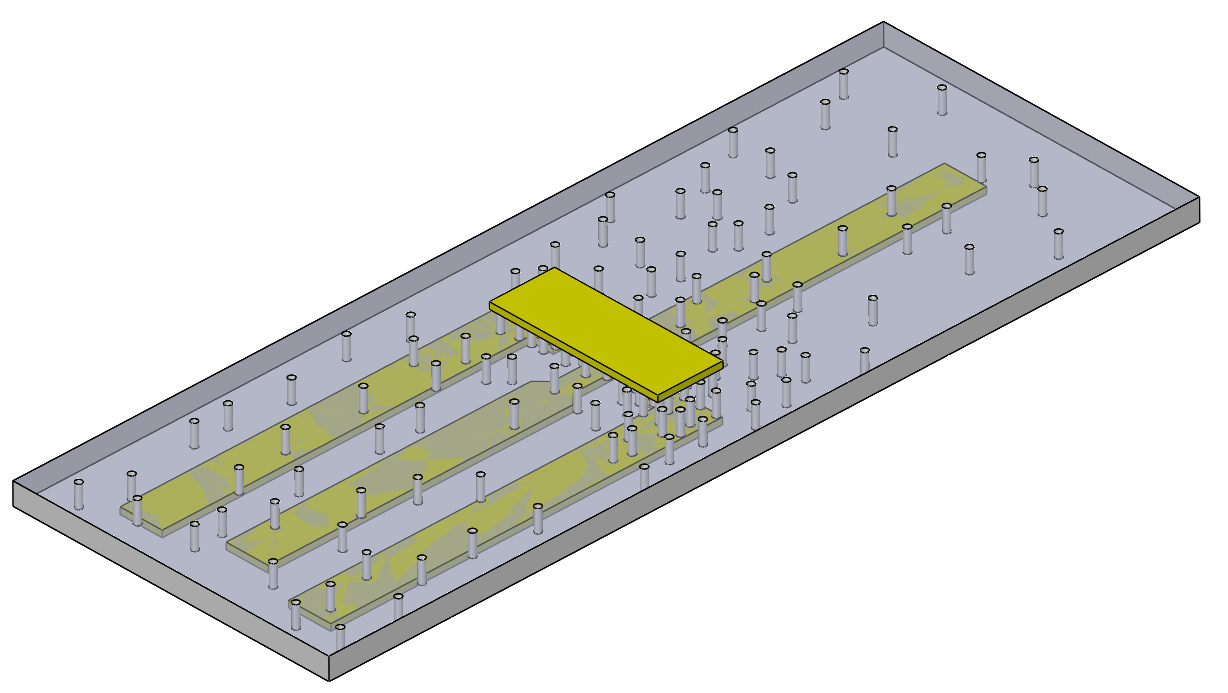
\includegraphics[scale = 0.35]{assets/figures/Court_circuit_B.png}
                  \caption{PVD d'or du court-circuit}
              \end{subfigure}
          \end{figure}
\end{itemize}

\section{Mesures du capteur sans amplificateur}
Plusieurs mesures ont été faites avec plusieurs types de paramètres. Toutes les mesures avec leurs paramètres ont été regroupées et sauvegardées
dans un document excel qui se trouve en annexe.\\
Chacune des mesures sur cet Excel est liée à un autre fichier contenant toutes les valeurs concernant cette mesure.
\begin{figure}[H]
    \centering
    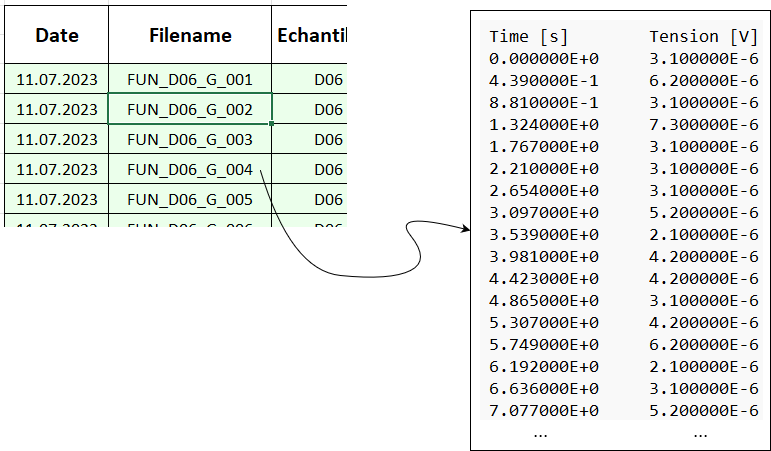
\includegraphics[scale = 0.4]{assets/figures/Data.png}
    \caption{Organisation des données}
    \label{fig:data_orga}
\end{figure}

Les mesures les plus significatives seront présentées dans ce rapport. \\

Des premières mesures ont été effectuées sans flux d'air. En effet, il est déjà intéressant d'observer le comportement du capteur
lorsque seulement le corps de chauffe est activé. Ce dernier est alimenté avec 15 mA. Les résultats sont les suivants :
\begin{figure}[H]
    \hspace{-0.5cm}
    \begin{subfigure}[b]{0.45\textwidth}
        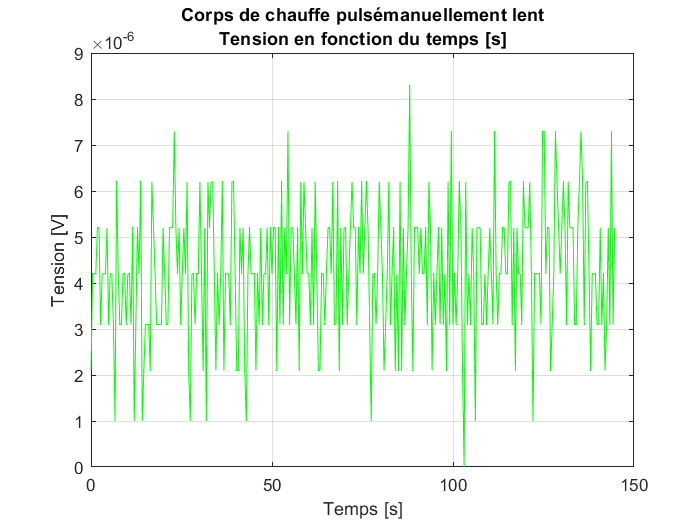
\includegraphics[scale = 0.45]{assets/figures/corps_chauffe_pulse_green.png}
        \caption{Support Design 5 - Corps de chauffe pulsé}
        \label{fig:chauffe_pulse_g}
    \end{subfigure}
    \begin{subfigure}[b]{0.45\textwidth}
        \includegraphics[scale = 0.45]{assets/figures/corps_chauffe_pulse_blue.png}
        \caption{Support Design 1 - Corps de chauffe pulsé}
        \label{fig:chauffe_pulse_b}
    \end{subfigure}
\end{figure}

Sur la figure \ref*{fig:chauffe_pulse_g}, aucun signal n'est distingable. En effet, il semble n'y avoir que du bruit. Cependant, sur la figure
\ref*{fig:chauffe_pulse_b}, la tension est bien moins stable. Pourtant aucune flux n'est encore ajouté. \\

La raison de ce phénomène peut se trouver dans le fait que chaque électrodéposition est faite à la main, une après l'autre. Ceci signifie que
les deux électrodépositions diffèrent certainement l'une de l'autre. \\
De plus, le corps de chauffe est assez proche des deux électrodépositions. De ce fait, il est probable que lorsqu'il est en marche, le corps de
chauffe transfert de la chaleur aux deux extrémités du capteur. Ces deux extrémités sont alors chauffées mais comme elles possèdent des nanofils
quelque peu différents d'un côté ou de l'autre, un gradient de température se forme et une certaine tension circule. \\
C'est une hypothèse du phénomène que l'on peut observer sur la figure \ref*{fig:chauffe_pulse_b}.\\

Le support Design 5 semble, lui, éviter ce transfert de chaleur. Cela peut être dû au fait qu'étant donné que la membrane est plaquée contre
la pièce du support, la chaleur transférée par le corps de chauffe est "perdue" dans la matière du support (ici : PLA).\\

Pour ces raisons, le support Design 1 a été privilégié étant donné qu'il semblait plus sensible que le support Design 5.\\

Par la suite, les mesures ont été poursuivies mais sans grand succès.

Un facteur a alors été modifé. Au lieu d'amener le flux d'air par une source d'air copmrimée, l'arrivée d'air sera effectué par une respiration humaine. Ceci nous a donné les résultats suivants :
\begin{figure}[H]
    \centering
    \begin{subfigure}[b]{0.45\textwidth}
        \includegraphics[scale = 0.43]{assets/figures/humanBreath_green_sansCorpsDeChauffe.png}
        \caption{Réponse du capteur à la respiration humaine - Design 5 - sans corps de chauffe}
        \label{fig:human_breath_green_without_heat}
    \end{subfigure}
    \begin{subfigure}[b]{0.45\textwidth}
        \includegraphics[scale = 0.43]{assets/figures/humanBreath_green_avecCorpsDeChauffe.png}
        \caption{Réponse du capteur à la respiration humaine - Design 5 - avec corps de chauffe}
        \label{fig:human_breath_green_with_heat}
    \end{subfigure}
\end{figure}

\section{Dépandances}
\section{Discussion}

\chapter{Conclusion}
%%if
Bien que non nécessaire dans un rapport de Bachelor, la discussion finale d'un projet résume les résultats obtenus et dresse une conclusion objective du projet. Un manager de société est souvent amené à lire de nombreux rapport, il ne s'intéresse généralement qu'à l'introduction au contexte de l'étude et à sa conclusion.

Si nécessaire, n'hésitez pas à scinder votre conclusion en deux parties : une conclusion technique et une conclusion personnelle.

Il est de coutume de signer la conclusion...
Pour conclure, reprenons les objectifs
%%fi

\section{Revue des objectifs}
\section{Résultats principaux}
\subsection{Délivrabes}
\subsection{Performances}
\section{Perspectives}

\vfil
\hspace{8cm}\makeatletter\@author\makeatother\par
\hspace{8cm}\begin{minipage}{5cm}
    %%if
    % Place pour signature numérique
    \printsignature
    %%fi
\end{minipage}

\clearpage

\printbibliography

\appendix
\appendixpage
\addappheadtotoc

%%if
\chapter{Première annexe}

Les annexes n'ont pas un contenu \underline{normatif} mais \underline{descriptif}. Tout contenu annexé ne doit pas être nécessaire à la bonne compréhension du travail.

Les annexes contiennent généralement :

\begin{itemize}
    \item les dessins mécaniques (mises en plan);
    \item les schémas électriques détaillés;
    \item des photographies du projet;
    \item des scripts et des extraits de code source;
    \item des documents techniques \pex \emph{datasheet};
    \item des développements mathématiques.
\end{itemize}
\section{Sous section}
\lipsum[1]
%%fi

\let\cleardoublepage\clearpage
\backmatter

\label{glossaire}
\printnoidxglossary
\label{index}
\printindex

% Le colophon est le dernier élément d'un document qui contient des notes de l'auteur concernant la mise en page et l'édition du document : il est parfaitement optionnel.
%%if
\clearpage
\Large\textbf{Colophon :}\par\normalsize
\thispagestyle{empty}
La qualité de cet ouvrage repose que le moteur \LaTeX. La mise en page et le format sont inspirés d'ouvrages scientifiques tels que le modèle de thèse de l'EPFL et celui des publications O'Reilly.

Les diagrammes et les illustrations sont édités depuis l'outil en ligne draw.io. Certaines illustrations ont été reprises dans Adobe Illustrator. Les représentations 3D sont exportées de SolidWorks et certains graphiques sont générés à la volée depuis un code source Python.

L'auteur fictive de ce document \emph{Maria Bernasconi} est un nom emprunté, par amusement, aux spécimens publiés par Postfinance.

Ce document a été compilé avec XeLaTeX.

La famille de police de caractères utilisée est \emph{Computed Modern} créée par Donald Knuth avec son logiciel METAFONT.
\vfil
Le Colophon est le dernier élément d'un document qui contient des notes de l'auteur concernant la mise en page et l'édition du document : il est parfaitement optionnel.
%%fi

\end{document}
